 % Este arquivo é uma adaptação do modelo LaTeX disponibilizado pelo UTUG (http://www.inf.ufrgs.br/utug/)
% Autor: Prof. Dr. Adriel M. Ziesemer Jr - IFRS Canoas
%
% Dica: Utilize o www.sharelatex.com para editar este documento. Utilize a opcão: Upload Zipped Project

%\documentclass[openright]{ifrs} % utilize openright para iniciar capítulos no anverso
\documentclass{ifrs}
\usepackage[T1]{fontenc}        % pacote para conj. de caracteres correto
\usepackage[utf8]{inputenc}     % pacote para acentuaçao
\usepackage{graphicx}           % pacote para importar figuras
\usepackage{times}              % pacote para usar fonte Adobe Times
\usepackage{listings}
\usepackage{multirow}           % pacote para usagrupar células em tabelas
\usepackage{scalefnt}           % pacote para redimensionar fontes em tabelas
\usepackage{amsmath}
\usepackage{rotating}           % pacote para rotacionar figuras
\usepackage{color,graphicx}     % pacote coloração
\usepackage{hyperref}           %links
\usepackage{subcaption}         %subfigure environment
\usepackage[table,xcdraw]{xcolor} %coloração de tabelas

\bibliographystyle{abnt}

% ensine o latex a separar em sílabas as palavras que eventualmente ele não souber
\hyphenation{en-si-na-men-tos a-gra-de-ci-men-to de-se-nha-dos}

\author{Fraga}{Kael V. de O.}

% edite o definicoes.sty se precisar alterar o nome do curso

\title{Pedal-to-Play: Um Sistema Web Gamificado para Monitoramento da Prática do Ciclismo}

\advisor[Prof.~Me.]{Pinto}{Rafael Coimbra}

\location{Canoas}{RS}

% palavras-chave (começar com letra maiúscula)
\keyword{Aplicativo de saúde e fitness}
\keyword{Geolocalização}
\keyword{Jogo pervasivo}
\keyword{Mobile}
\keyword{Web}

% nominata
\newcommand{\nominata}{
%    \MakeUppercase{\instituicao}\\
%    Reitor: Prof. Osvaldo Casares Pinto\\
%    Diretor do Instituto: Prof. Dr. Mariano Nicolao\\
%    Coordenadora do curso: Prof\textsuperscript{a}. Patrícia Nogueira %H\"{u}bler\\
%    Bibliotecária-chefe: Sabrina Eufrasio
}

% inicio do documento
\begin{document}

% folha de rosto
\maketitle

% Dedicatoria (opcional)
\clearpage
\begin{flushright}
\mbox{}\vfill
{\sffamily\itshape
"A day without laughter is a day wasted."\\
Charlie Chaplin}
\end{flushright}


% Agradecimentos (opcional)
\chapter*{Agradecimentos}  \label{cap:agradecimentos}
Primeiramente, gostaria de agradecer a meu orientador Rafael Coimbra Pinto, pelo tempo e reforços investidos, pelas ideias compartilhadas, por não me desencorajar em nenhum momento desta trajetória e acreditar na conclusão deste projeto. 
\par
Agradeço a todos os professores do Câmpus Canoas, dos quais eu tive o privilégio de ser aluno, pois cada um, de alguma forma, contribuiu com os conhecimentos necessários para a realização deste trabalho.
\par
Agradeço a minha família, amigos e colegas de trabalho, por compreenderem todas as vezes que eu não estive presente por estar envolvido neste projeto, pelas palavras de encorajamento, por serem voluntários para experimentar o sistema, fornecerem \textit{feedback} e ideias. 
\par
Para concluir, agradeço especialmente a minha mãe, Ceila Adriany, companheira de pedaladas e que nunca deixou de acreditar que eu conseguiria.

% Resumo
%Arquivo contendo os Resumos
\begin{abstract}
O presente trabalho apresenta o desenvolvimento de um aplicativo "gamificado"\ com a pretensão de motivar seus usuários a praticarem a atividade de ciclismo. A popularização crescente dos \textit{smartphones} e \textit{tablets} trouxe consigo os aplicativos voltados para a saúde pessoal e condicionamento físico. Eles pretendem servir como ferramentas de auxílio ao usuário na prática de uma atividade física, em um cenário em que possuir uma rotina sedentária é comum e a prática constante de exercícios perde espaço. Um aplicativo que usa técnicas de gamificação tem a aspiração de motivar com mais eficiência um usuário que deseje persistir praticando uma atividade física, pois essas técnicas se apropriam dos elementos-chave que os jogos empregam para envolver o ser humano: a socialização, a competição, a fuga da realidade e o aprendizado. Ao longo deste trabalho são descritos os conceitos envolvidos para elaboração do projeto; trabalhos relacionados na mesma temática, os métodos para pesquisa, análise, projeto e desenvolvimento do \textit{software}; as tecnologias implementadas voltadas para Web, incluindo os \textit{frameworks} AngularJS e Bootstrap; o desenvolvimento para \textit{mobile} usando Cordova; o desenvolvimento do \textit{web service} REST com Slim; o uso de geolocalização para monitorar pedaladas do usuário; o módulo de avatar virtual; o módulo de desafios e recompensas e os \textit{softwares} terceiros agregados. Concluindo, são apresentados os resultados obtidos após a implementação da solução técnica, contendo \textit{print screens} das funcionalidades do \textit{software}, os testes envolvendo sessões reais de ciclismo e os objetivos cumpridos. 
\end{abstract}

\begin{englishabstract}
{Pedal-to-Play: A Gamified Web Application to Track Bicycle Rides}
{Health and Fitness application. Geolocation. Pervasive Game. Mobile}

This paper presents the development of a gamified application intended to motivate its users to practice cycling activity. The growing popularity of smartphones and tablets brought applications focused on health and  fitness. They plan to serve as tools in order to aid the user to practice a physical activity, in a scenario that maintaining a sedentary routine is common and practicing exercises loses ground. An application that implements gamification techniques aspires to motivate more efficiently an user that wishes to persist practicing a physical activity, because these techniques take ownership of the key elements that games employ to engage the human being: socializing, competition, escape from reality and learning. Throughout this paper are described the concepts involved in this project development; works related to the same theme, the methods of research, analysis, project design and development of software; the implemented technologies for Web, including the frameworks AngularJS and Bootstrap; development for mobile devices using Cordova; REST web service development with Slim; the use of geolocation to track user rides; the virtual avatar module; the challenges and rewards module and third party softwares aggregated. After the implementation of the technical solution, the results obtained are presented, containing print screens of software features, tests involving real rides and achieved goals.
\end{englishabstract}

% lista de abreviações
% Arquivo contendo a lista de abreviaturas e siglas
\begin{listofabbrv}{SPMD}
        \item[AJAX] Asynchronous Javascript and XML 
        \item[API] Application Programming Interface 
        \item[ASP] Active Server Pages
        \item[CORS] Cross Origin Resource Sharing
        \item[CSS] Cascading Style Sheets
        \item[DAO] Data access object
        \item[GPS] Global Positioning System 
        \item[GUI] Graphical User Interface
        \item[HTML] Hyper Text Markup Language
        \item[HTTP] Hypertext Transfer Protocol
        \item[IE] Internet Explorer
        \item[Java EE] Java Enterprise Edition
        \item[JS] JavaScript
        \item[JSON] JavaScript Object Notation
        \item[JSP] JavaServer Pages 
        \item[MVC] Model-View-Controller
        \item[PHP] PHP: Hypertext Preprocessor
        \item[REST] Representational State Transfer
        \item[SOAP] Simple Object Access Protocol
        \item[SGDB] Sistema de Gerenciamento de Banco de Dados
        \item[SSH] Secure Shell
        \item[SVG] Scalable Vector Graphics
        \item[UML] Unified Modeling Language
        \item[URL] Uniform Resource Locator
        \item[W3C] World Wide Web Consortium
        \item[WLAN] Wireline Local Area Network
        \item[XML] eXtensible Markup Language
\end{listofabbrv}

% lista de figuras
\listoffigures

% lista de tabelas
\listoftables

% sumário
\tableofcontents

% Introdução
%Arquivo contendo o capítulo Introdução
\chapter{Introdução} \label{cap:introducao}
Atualmente, \textit{smarthphones} e aplicativos para acompanhamento de atividades físicas e saúde pessoal estão bem popularizados, eles buscam motivar seus usuários a continuar praticando exercícios e dedicando tempo de suas vidas para saúde. Todavia, esses resultados não são instantâneos e nesta época de bombardeio de informações, o \textit{feedback} demorado da prática de um exercício vem a desmotivar os iniciantes, entre outros fatores, como tais: a exaustiva rotina diária e a falta de acompanhamento para a atividade. \par 

Nestes pontos fracos que os aplicativos modernos de acompanhamento de atividades físicas atacam, se tornando companheiros de bolso para qualquer um que deseje praticar um esporte, mesmo que por lazer. Eles proporcionam a socialização através das redes sociais, \textit{feedback} instantâneo através dos dados coletados via funcionalidades dos \textit{smarthphones} e competição por melhores desempenhos entre os usuários do mesmo aplicativo. \par

O modo de vida contemporâneo é outro fator que não favorece a prática de exercícios físicos, pois a maior parte do dia da população é ocupada por trabalho ou estudo, senão ambos. Entre estes dois também há o quesito trânsito. O tempo livre restante é aproveitado para descanso ou socialização com família ou com amigos. Aqueles que praticam esportes por \textit{hobbie} encontram, ao passar o tempo, cada vez mais obstáculos para praticá-los: seja por falta de tempo, por problemas econômicos e financeiros ou por simplesmente não sentir prazer na atividade praticada \cite{butcher2002, liz2013}. \par

Vivendo neste cenário, onde a prática de uma atividade física não se torna hábito em nossas vidas (embora seja necessário para manter nosso corpo e mente saudáveis) surge o questionamento, de que maneira um \textit{software} poderia motivar os usuários a persistirem na prática de um exercício, mais especificamente, a atividade de ciclismo? \par

Assim, a pesquisa fruto desse projeto pretende desenvolver um \textit{software} multiplataforma (\textit{mobile} e \textit{desktop}) que use as tecnologias de desenvolvimento \textit{Web} e aplique conceitos de gamificação no formato de um jogo pervasivo, o qual será denominado Pedal-to-Play. \par

Entre as funcionalidades do Pedal-to-Play, propõe-se a captura e processamento de determinados dados durante as seções de ciclismo do usuário, com o fim de mensurar o desempenho dele na atividade, recompensando-o com pontos e \textit{badges} (troféus virtuais e indicadores de realização de tarefas) de acordo com os resultados alcançados. Pretende-se possibilitar o compartilhamento das recompensas em redes sociais. O \textit{software} também possuirá um sistema de \textit{avatar} virtual customizável, o qual ilustrará o perfil do usuário, contendo informações sobre a evolução do mesmo na atividade de ciclismo.

\section{Motivação}
Diferente dos \textit{softwares} que somente coletam os dados do usuário e os exibem de forma gráfica, um sistema que implementa técnicas de gamificação em seu desenvolvimento propõe alternativas para a superação de fatores desmotivadores na prática de uma atividade. As técnicas de gamificação  trabalham estimulando os principais fatores motivadores para o ser humano: competição, aprendizado, fuga da realidade e interação social \cite{vianna2013}. Assim, o Pedal-to-Play proporá desafios ao usuário e o mesmo será recompensado pela participação neles. Buscando concomitantemente conciliar o entretenimento na atividade exercida pelo usuário e permitindo a socialização com outros ciclistas que também façam uso do \textit{software}. \par

A atividade de ciclismo foi escolhida como foco do trabalho pelos benefícios a saúde do praticante, ao meio ambiente e a mobilidade urbana. \citet{rojasrueda2011} constatou que o aumento de adeptos à bicicleta como meio de transporte na cidade de Barcelona ocasionou na diminuição de acidentes no trânsito e a diminuição de gás carbônico no ambiente.

\section{Objetivo}
Este trabalho possui os seguintes objetivos:

\subsection{Objetivo Geral}
Desenvolver um \textit{software} com a pretensão de motivar o usuário a persistir praticando a atividade de ciclismo. 

\subsection{Objetivos Específicos}
\begin{itemize}
\item Identificar quais dados devem ser analisados e como computá-los para mensurar o desempenho do ciclista;
\item Identificar e selecionar quais \textit{frameworks} e linguagens de programação adequados para o desenvolvimento do \textit{software};
\item Desenvolver uma interface homem-computador responsiva e multiplataforma;
\item Desenvolver um mecanismo dentro da aplicação para propor desafios ao usuário e recompensá-lo pela participação nestes;
\item Permitir ao usuário compartilhar seus dados contidos no \textit{software} em redes sociais;
\item Analisar e aplicar técnicas de gamificação para o desenvolvimento do \textit{software}.
\end{itemize}

\section{Organização do Texto}
Este documento está divido em três capítulos. O capítulo \ref{cap:metodologia} versa os métodos que serão utilizados para a elaboração da pesquisa e o desenvolvimento do \textit{software}, assim como descreve as etapas do trabalho e as funcionalidades que pretende-se implementar. O capítulo \ref{cap:cronograma} conterá uma tabela contendo as tarefas fundamentais deste trabalho e em qual mês cada uma delas será efetuada.
O cronograma abrange quatro meses do segundo semestre de 2015.



% Revisao Bibliográfica
%Arquivo contendo o capítulo Revisão Bibliográfica
\chapter{Revisão Bibliográfica} \label{cap:revbib}
Esse capítulo tem como objetivo descrever os principais conceitos apresentados para o desenvolvimento do \textit{software} proposto. Os conceitos envolvidos são: jogo pervasivo; gamificação; desenvolvimento multiplataforma; aplicativos de saúde e \textit{fitness}; avatares virtuais e geolocalização.

\section{Jogos Pervasivos}
Um jogo pervasivo é um tipo de jogo digital, no qual ao menos uma interação do usuário com o sistema transcorre no universo físico. Eles integram os aspectos físicos e sociais do mundo real em jogos digitais, estendendo a interação do jogador com o jogo, pois em ambientes virtuais a interface com o usuário está limitada ao uso dos periféricos do computador. Os recentes dispositivos celulares (\textit{smartphones}) e a popularização de tecnologias de rede sem fio 
(tais como, \textit{WiFi\footnote{WiFi é o termo popular para redes sem fio ethernet padrão  WLANs (Wireline Local Area Networks) \cite{lehr2003}.} e 3G\footnote{3G refere-se a terceira geração de serviços de dados móveis, fornecido por operadoras provedoras de redes móveis \cite{lehr2003}.}}) facilitam a extensão das interfaces homem-computador. \cite{magerkurth2005, vianna2013}. Um exemplo de jogo pervasivo é o Human Pacman. \par

\begin{figure}[h]
    \caption[Processo de coleta de um item no Human Pacman]{Processo de coleta de um item no Human Pacman \cite{cheok2003}.}
    \centerline{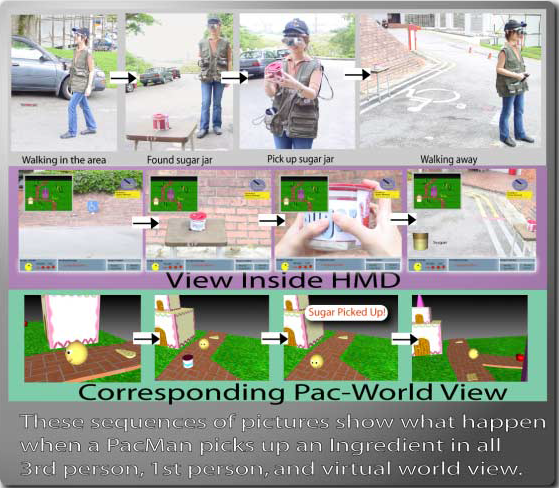
\includegraphics[width=20em]{figuras/humanpacman.png}}
    \label{fig:humanpacman}
\end{figure}

No Human Pacman, os jogadores interpretam o papel dos personagens do jogo Pac-Man no mundo real, enquanto vestem-se com trajes customizados integrados a dispositivos eletrônicos. Esses trajes permitem interação entre os jogadores via WiFi e interação com o sistema que insere elementos virtuais no mundo físico, através de técnicas de realidade aumentada, como ilustrado na figura \ref{fig:humanpacman} \cite{cheok2003}. 

\section{Gamificação}
A gamificação (do original em inglês \textit{gamification}) consiste na aplicação de mecanismos de jogos com o intuito de resolver problemas práticos ou motivar um público específico a realizar certas atividades em contextos fora de jogos. Alguns exemplos de aplicação de gamificação tem como objetivo: agilizar processos de aprendizagem ou treinamento; tornar mais agradáveis tarefas consideradas tediosas ou repetitivas; motivar usuários a reforçar a condição física e emocional e até usar jogos em forma de propagandas de produtos e serviços. O Duolingo\footnote{\url{https://www.duolingo.com/}} é um exemplo de \textit{software} "gamificado" para agilizar processos de aprendizagem de uma língua estrangeira e o SuperBetter\footnote{\url{https://www.superbetter.com/}}, para incentivar o usuário a reforçar o condicionamento físico. \cite{vianna2013, zichermann2011}.

\section{Desenvolvimento Multiplataforma}
Com a intenção de garantir que o \textit{software} possua portabilidade para plataformas \textit{mobile} e \textit{desktop} se fará uso do desenvolvimento \textit{Web}. Segundo \citet{lopes2013}, o desenvolvimento \textit{Web} é democrático, aberto e acessível, pois praticamente, todo dispositivos possui um navegador (\textit{web browser}). Uma aplicação \textit{Web} garante acesso a um número maior de usuários do que uma aplicação nativa para um determinado dispositivo. Lopes também salienta que é cada vez mais comum usar as linguagens fundamentais da \textit{Web} para desenvolver aplicativos \textit{mobile}. A subseção seguinte versará sobre as tecnologias fundamentais do desenvolvimento \textit{Web}.

\subsection{Lado do Cliente}
As tecnologias fundamentais usadas em sistemas \textit{Web}, no lado do cliente, são o HTML (\textit{Hyper Text Markup Language}), o CSS (\textit{Cascading Style Sheets}) e o JavaScript (JS). \par

HTML5 é a versão atual do HTML, linguagem de marcação para escrever a estrutura principal de páginas \textit{Web}. HTML fornece instruções aos \textit{web browsers} (exemplos: Chrome, IE, Firefox) sobre o que exibir em uma página. Cada conteúdo é representado por um conjunto de elementos pré-definidos chamados \textit{tags} \cite{html5}. \par 

CSS é a linguagem usada para definir o estilo e o \textit{layout} do conteúdo de uma página HTML. Ela também permite ajustar o \textit{layout} das aplicações para qualquer tamanho de tela, inclusive o \textit{mobile}. Esta característica é importante para o \textit{software} desde trabalho, o qual pretende ser multiplataforma. A versão atual do CSS é o CSS3 \cite{css3}. \par
 
JS é uma linguagem de programação interpretada e orientada a objetos, usada para manipular o comportamento de páginas HTML. Possui recursos para alterar o conteúdo das páginas, o estilo delas e validar entradas do usuário. \cite{javascript}. \par

No desenvolvimento do lado do cliente também podem ser empregados \textit{frameworks} e bibliotecas. Estes se propõem a facilitar o uso das linguagens listadas anteriormente, assegurar questões de compatibilidade entre navegadores, assegurar questões de segurança e confiabilidade e de portabilidade para diferentes dispositivos. \par

Os seguintes \textit{frameworks} serão investigados para o possível uso no desenvolvimento do \textit{software} deste trabalho: Bootstrap\footnote{\url{http://getbootstrap.com/}}, para desenvolvimento de páginas \textit{Web} responsivas e adaptáveis para dispositivos com tamanhos diversos; AngularJS\footnote{\url{https://angularjs.org/}}, usado para tornar páginas HTML estáticas em páginas dinâmicas, estendendo o vocabulário do HTML; e jQuery\footnote{\url{https://jquery.com/}}, usado para facilitar e estender o JS. \par
 
A plataforma Cordova\footnote{\url{https://cordova.apache.org/}}, para conversão de sistemas \textit{Web} em aplicações nativas \textit{mobile}, também será investigada. Ela permite atribuir ao \textit{software} acesso aos recursos de \textit{hardware} dos dispositivos \textit{mobile}.

\subsection{Lado do Servidor} \label{sec:server}
Atualmente o pódio das tecnologias para o desenvolvimento \textit{Web} do lado do Servidor está ocupado pelo PHP, em primeiro lugar; ASP.NET em segundo e o Java, em terceiro \cite{w3techs2015}. \par

Java \textit{Web} consiste na implementação das APIs de Servlets e JavaServer Pages (JSP). Servlet é a tecnologia usada pelo Java para geração de páginas HTML dinâmicas, são classes Java com HTML embutido. Páginas JSP consistem no inverso, são estruturadas como páginas HTML com código Java embutido. Servlets e JSP podem ser desenvolvidos na plataforma Java Enterprise Edition (Java EE). A Java EE consiste em um conjunto de especificações para várias APIs de desenvolvimento Java para \textit{Web} \cite{basham2008}. Os pontos fortes do Java \textit{Web} estão na portabilidade para diferentes plataformas de \textit{hardware}, banco de dados e servidores e a grande quantidade de \textit{frameworks} existentes, tais como Primefaces\footnote{\url{http://www.primefaces.org/}} e Spring\footnote{\url{http://spring.io/}}. \par

ASP.NET é uma tecnologia da Microsoft, parte do .NET \textit{Framework} para desenvolvimento de aplicações \textit{Web}. O desenvolvimento com ASP.NET pode ser feito com qualquer linguagem compatível com o .NET. Algumas das vantagens desta tecnologia envolvem a separação clara entre a interface do usuário e a lógica de programação; a familiaridade com o desenvolvimento \textit{desktop}; a ferramenta de desenvolvimento Visual Studio, com diversos recursos para facilitar o trabalho do desenvolvedor e a integração com todos os recursos do \textit{framework} .NET \cite{imar2014}. As desvantagens do ASP.NET são: sua limitação ao sistema operacional Windows e a licença de uso do Visual Studio não ser gratuita. \par

PHP é uma linguagem de programação presente em 10 milhões de sites no mundo inteiro. O PHP adiciona dinamismo às páginas estáticas e automatiza tarefas, diminuindo mão-de-obra. Possui portabilidade para várias plataformas \textit{desktop} (exemplos: Linux, Unix e Windows); possui código aberto e licença de uso gratuita; suporta vários bancos de dados (entre eles: MySQL, Oracle e PostgreSQL). Sua versão mais recente é o PHP 5 \cite{niederauer2004, welling2003}. \par

Outros pontos fortes do PHP envolvem sua alta performance (um único servidor pode lidar com milhões de acessos por dia); bibliotecas nativas para várias tarefas comuns na \textit{Web} (funções para gerenciamento de imagens, conexão com \textit{web services}, interpretação de XML, envio de \textit{email}, gerenciamento de \textit{cookies} e geração de documentos PDF); fácil aprendizado (a sintaxe de PHP é baseada em outras linguagens, entre elas, C e Perl); suporte ao desenvolvimento orientado a objetos e disponibilidade de suporte técnico \cite{welling2003}. \par

Pretende-se usar a linguagem PHP para desenvolvimento do lado do servidor, pois comparado com as outras duas principais linguagens (ASP.NET e Java) o PHP se destaca por sua licença gratuita, portabilidade e suporte nativo (sem \textit{frameworks}) a funcionalidades que serão essenciais no software deste trabalho, tais como: gerenciamento de imagens, interpretação de arquivos JSON e acesso a banco de dados. \par

No quesito sistemas de gerenciamento de bando de dados (SGDB), os três mais usados atualmente segundo o \textit{site} da DB-Engines são o Oracle em primeiro lugar, o MySQL em segundo e o Microsoft SQL Server em terceiro. O MySQL possui licença de uso \textit{open source} e versão gratuita sem restrições, enquanto o Oracle e o Microsoft SQL Server são \textit{softwares} com licença de uso comercial, por estes motivos pretende-se fazer uso dele. \par

\section{Aplicativos de Saúde e \textit{Fitness}}
Aplicativos de Saúde e \textit{Fitness} são \textit{softwares} desenvolvidos para dispositivos \textit{mobile} com o objetivo de estimular o usuário a praticar atividades benéficas à saúde e ao bem-estar \cite{bonome2012}. Alguns exemplos dessa categoria de aplicativos são o Strava\footnote{\url{https://www.strava.com/}} e o  Runtastic\footnote{\url{https://www.runtastic.com/}}. \par

\section{Avatares Virtuais}
Avatares são corpos virtuais criados para representar a identidade e ações de um usuário em um mundo virtual. Eles são usados como ferramentas de comunicação e para representar visualmente os usuários. Uma das principais características dos avatares é a sua customização, orientada pelo desejo de quem o cria \cite{ducheneaut2009}. Um exemplo de aplicativo específico para criação de avatares e utilização destes como ferramente de socialização entre os usuários é o \textit{BuddyPoke}, ver figura \ref{fig:avatar}. \par

\begin{figure}[hb]
    \caption{Exemplo de avatar criado no aplicativo BuddyPoke.}
    \centerline{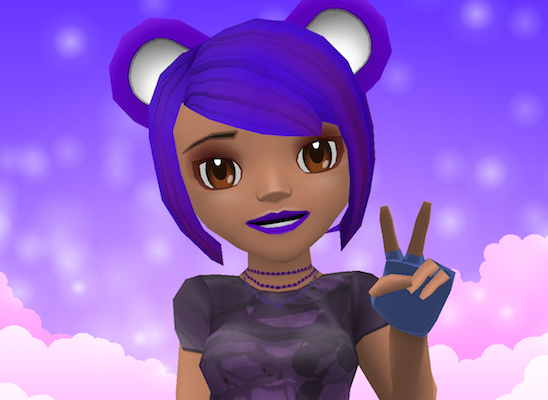
\includegraphics[width=17em]{figuras/avatar.png}}
    \label{fig:avatar}
\end{figure}
\centerline{Fonte: Página oficial do BuddyPoke na \textit{Web}\footnote{Disponível em: <\url{http://www.buddypoke.com/}>. Acesso em jun. 2015.}}

\section{Geolocalização}
Geolocalização é o termo usado para descrever o posicionamento geográfico de um objeto no planeta, a partir de seus valores de latitude e longitude \cite{aires2014}. Essas coordenadas são obtidas utilizando \textit{Global Positioning System} (GPS), um sistema desenvolvido e mantido pelas Forças Aéreas dos Estados Unidos. Este sistema consiste em três segmentos: o espacial, composto por 24 satélites operantes em órbita e transmitindo sinais de radio; o controle, o qual consiste nas estações de controle que mantêm os satélites funcionando adequadamente; e o segmento do usuário, o qual compreende os aparelhos receptores dos sinais vindos dos satélites \cite{gpsgov}. O funcionamento do GPS é ilustrado na figura \ref{fig:gps}. \par

\begin{figure}[h]
    \caption[Funcionamento do GPS]{Funcionamento do GPS \cite{cesani2013}.}
    \centerline{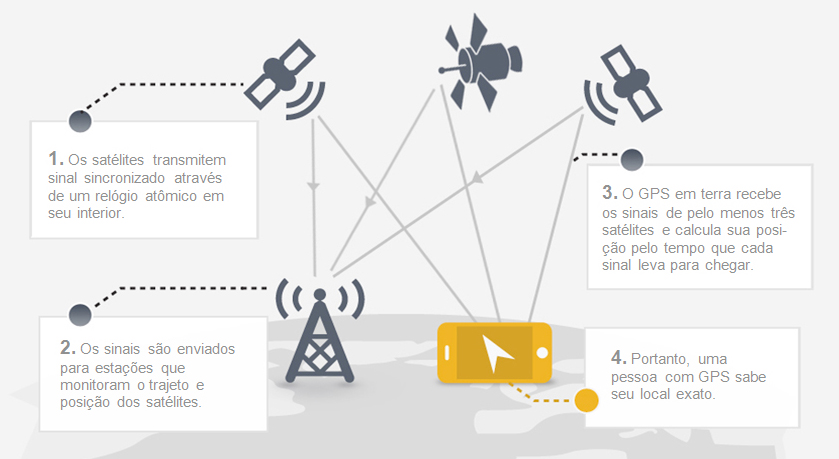
\includegraphics[width=30em]{figuras/gps.png}}
    \label{fig:gps}
\end{figure}

No entanto, o uso de GPS tem suas limitações. Segundo \citet{sukaphat2013}, os sinais de GPS possuem um alcance limitado e uma capacidade baixa de atravessar barreiras. Estas características impedem o funcionamento adequado desta tecnologia em ambientes fechados. \par

%\section{Conclusões}
%Reunir as ideias principais abordadas no capítulo.

% Estado da Arte
%Arquivo contendo a sessão Estado da Arte
\chapter{Estado da Arte} \label{cap:estadoarte}
Nesta seção serão descritos alguns trabalhos relacionados com a temática e conceitos do Pedal-to-Play. Eles serão divididos em dois grupos: aplicativos comerciais e trabalhos científicos.

\section{Aplicativos comerciais}
Entre os aplicativos comerciais mais populares atualmente na categoria de Saúde e \textit{Fitness}, com a atividade de ciclismo como um dos focos, estão o Strava e o Runtastic Road Bike. Ambos utilizam funções do geolocalização para traçar rotas, guardar trajetos do usuário e calcular valores de velocidade, altitude e distância percorrida, com a intenção de gerar relatórios sobre o desempenho do usuário em corridas ou pedaladas. As Figuras \ref{fig:strava} e \ref{fig:Runtastic} são \textit{print screens}, respectivamente, dos aplicativos Strava e Runtastic Road Bike.\par 

\begin{figure}[h]
\centering
\begin{minipage}{.5\textwidth}
  \centering
  \captionof{figure}{Rastreamento de pedalada\\do Strava.}
  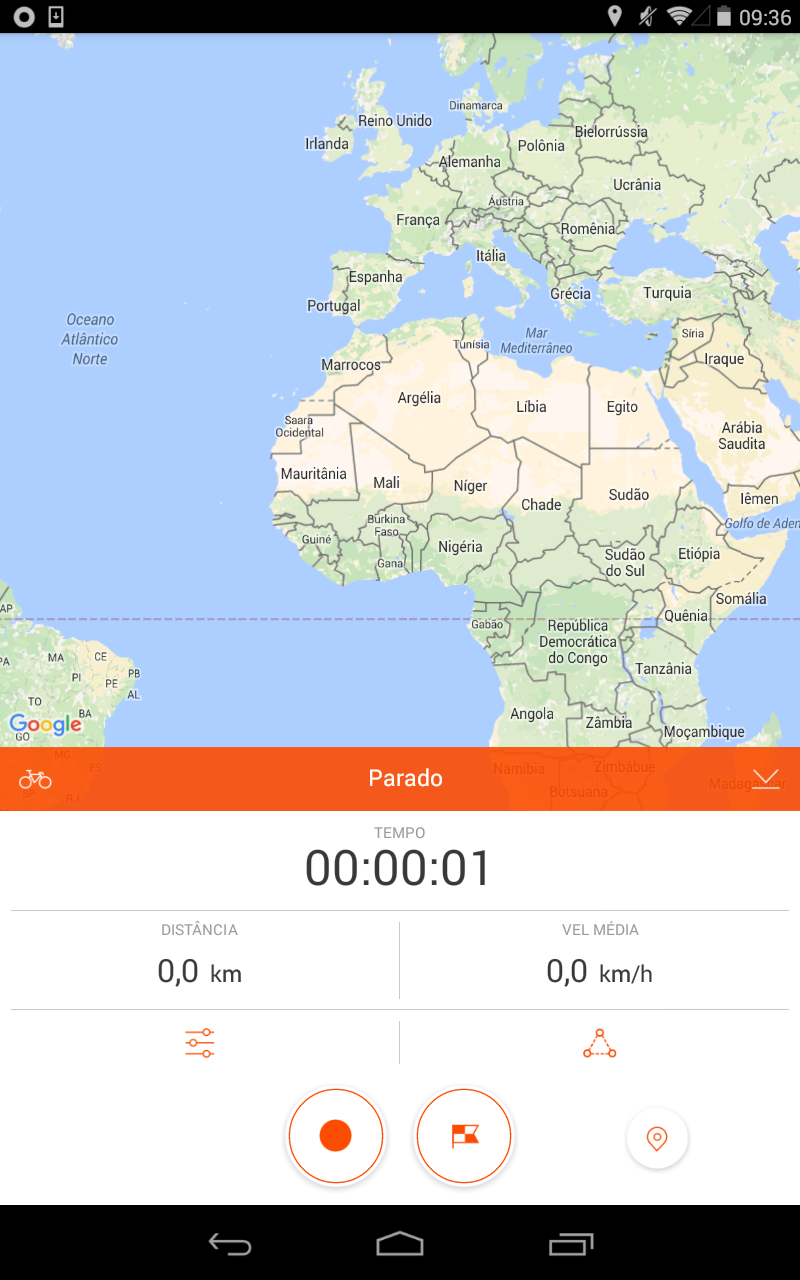
\includegraphics[width=.8\linewidth]{figuras/strava.png}
  \label{fig:strava}
  \newline
\end{minipage}%
\begin{minipage}{.5\textwidth}
  \centering
  \captionof{figure}{Histórico de atividades\\do Runtastic Road Bike.}
  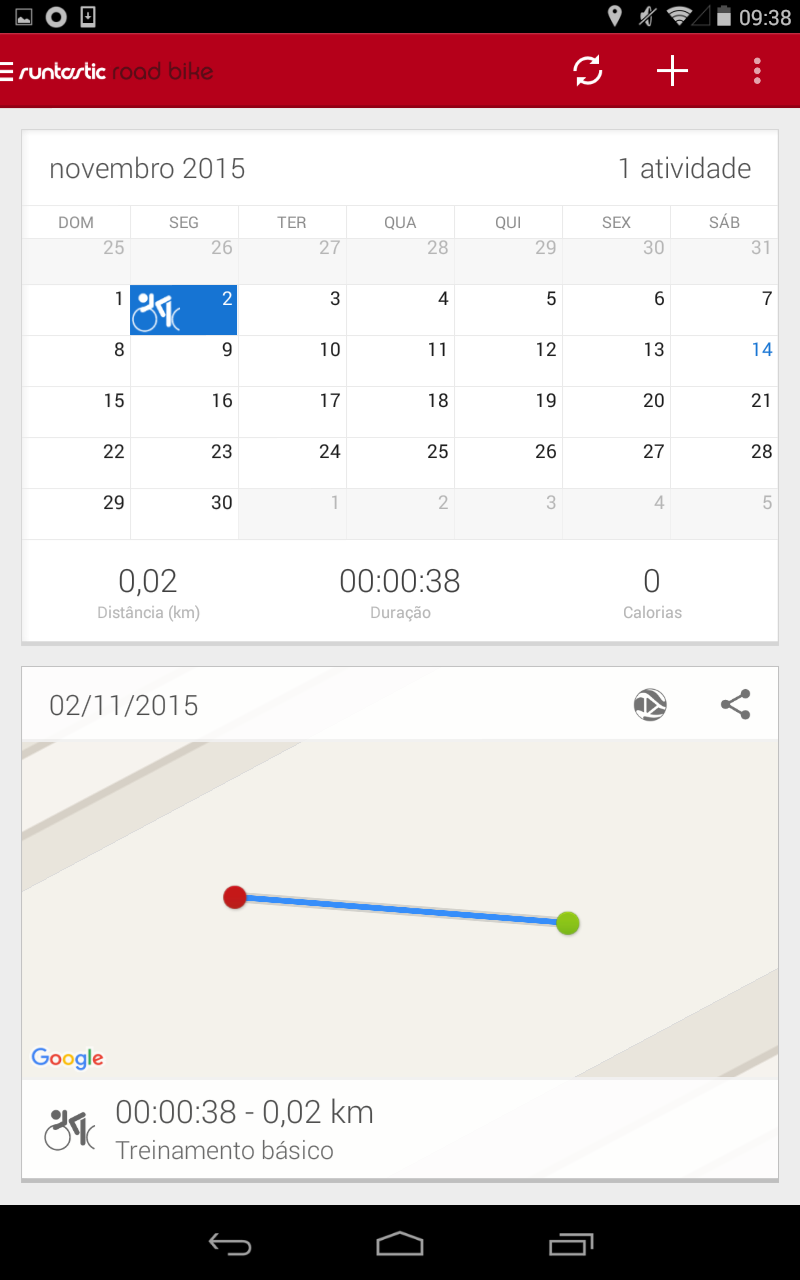
\includegraphics[width=.8\linewidth]{figuras/Runtastic.png}
  \label{fig:Runtastic}
  \newline
\end{minipage}
\centerline{Fonte: \textit{print screens} das aplicações Strava e Runtastic Road Bike, respectivamente.}
\end{figure}

O Strava, em particular, utiliza alguns conceitos de gamificação, tais como: sistema de desafios e recompensas (baseadas em prêmios, \textit{ranking} e \textit{badges}); criação de metas e socialização entre usuários. \par 

Estes aplicativos também possibilitam integração com redes sociais e compartilhamento de dados entre os usuário. Assim como o interfaceamento com outros dispositivos eletrônicos para monitoramento de atividades, tal como o Garmin\footnote{\url{http://www.garmin.com/}} (Figura \ref{fig:garmin}). \par 

\begin{figure}[h]
    \caption{Computador compacto para bicicleta com GPS da Garmin.}
    \centerline{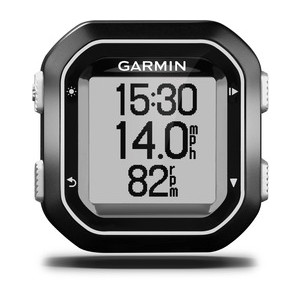
\includegraphics[width=11em]{figuras/cf-lg.jpg}}
    \label{fig:garmin}
\end{figure}
\centerline{Fonte: Página oficial do produto na Web\footnote{Disponível em:  <\url{https://buy.garmin.com/pt-BR/BR/cIntoSports-cCycling-p1.html}>. Acesso  em jun. 2015.}}

\section{Trabalhos científicos}
Entre os trabalhos científicos pesquisados estão as obras de Cesani e Dranka \citeyearpar{cesani2013} e Rosero \citeyearpar{gaidos2012}, ambos propuseram sistemas para auxiliar ciclistas em suas atividades. \par

Cesani e Dranka propuseram diretrizes para o desenvolvimento de uma aplicação \textit{mobile} com a intenção de auxiliar os ciclistas de Curitiba em seus trajetos. Para isso, eles estudaram o sistema de navegação GPS; as ciclovias e vias alternativas de Curitiba; o perfil do ciclista desta cidade; documentos sobre a infraestrutura urbana cicloviária e produtos relacionados usados pelos ciclistas de Curitiba. Como resultados, os autores definiram a fundamentação teórica da pesquisa e uma base para o desenvolvimento da interface homem-computador para um futuro protótipo funcional. \par

Rosero, em sua dissertação de mestrado, desenvolveu um protótipo para um sistema de treinamento e monitoramento para ciclistas (Figura \ref{fig:rosero}). Envolvendo a implementação de uma aplicação para plataforma Android e módulos de \textit{hardware} (tais como um módulo Bluetooth\footnote{Bluetooth é uma tecnologia de comunicação sem fio, baseada em ondas de rádio frequência de curto alcance. Possibilita comunicação eficiente e eficaz entre diferentes dispositivos eletrônicos \cite{gaidos2012}.}, sensores de frequência cardíaca, de percentual de oxigênio e de temperatura). Este sistema fornece informações dos sinais fisiológicos do usuário, processando e disponibilizando estas na rede social Twitter\footnote{\url{https://twitter.com}}, para que um treinador possa acompanhar os resultados.

\begin{figure}[t]
    \caption[Protótipo de \textit{hardware} desenvolvido por Rosero ligado ao capacete de um ciclista]{Protótipo de \textit{hardware} desenvolvido por Rosero ligado ao capacete de um ciclista \cite{gaidos2012}.}
    \centerline{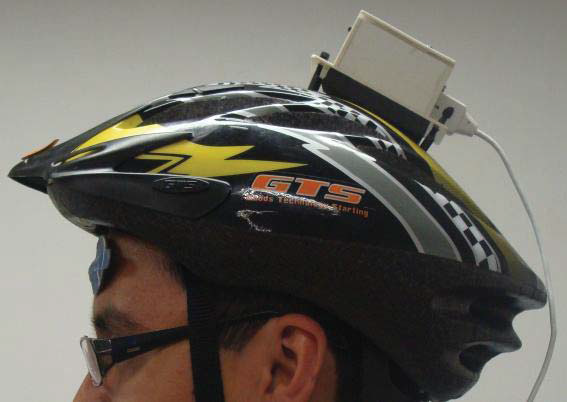
\includegraphics[width=18em]{figuras/rosero.png}}
    \label{fig:rosero}
\end{figure}

\section{Conclusões}
Neste capítulo foram apresentados trabalhos e sistemas existentes relacionados a temática e proposta do Pedal-to-Play. Um fator comum notável entre estes sistemas é que o público alvo são pessoas no geral já adeptas ao ciclismo, as quais o praticam por hábito e lazer ou como esporte. O projeto de Rosero foca no treinamento de ciclistas, usando um \textit{hardware} e \textit{software} personalizados para atender as necessidades destes e o trabalho de Cesani e Dranka é voltado para usuários que já utilizam a bicicleta como meio de locomoção em Curitiba. Nos aplicativos Strava e Runtastic, os usuários com maior visibilidade são aqueles que se dedicam integralmente ao esporte (o alto desempenho na atividade resulta em \textit{ranking} alto e vários \textit{badges}). O Pedal-to-Play por sua vez, ao se propor a trazer elementos de jogos à prática de ciclismo, foca também nas pessoas que têm mais familiaridade com \textit{video games} do que com o esporte (o exemplo clássico usado por Jane
McGonigal (\citeyearpar{mcgonigal2011reality}) sobre o quanto as pessoas têm se dedicado aos \textit{video games} é o do jogo \textit{online} \textit{World of
Warcraft}, ao somar todas as horas jogadas exclusivamente nele o resultado seria de 5,93 bilhões de anos, somente entre os anos de 2004 e 2011). O projeto visa  disponibilizar um ambiente cativante e motivador, também para este público não praticante envolver-se no ciclismo e torná-lo um hábito. No próximo capítulo será apresentado como a ideia do Pedal-to-Play foi projetada e desenvolvida.

% Desenvolvimento
\chapter{Análise e Projeto} \label{cap:espec}
% Introduzir capítulo, falar sobre análise e modelagem.
Este capítulo versa sobre a modelagem e planejamento do sistema. As próximas seções apresentarão a arquitetura do sistema, apresentando os componentes dele e suas relações; os requisitos, levantando as restrições técnicas e necessidades; a definição dos casos de uso, baseada nos objetivos do projeto e funcionalidades propostas; a prototipação das interfaces, a qual contemplará a comunicação entre usuário e sistema e por fim, a definição do modelo de entidade relacionamento, no qual o banco de dados será estruturado.  

\section{Arquitetura}
% explicar Cliente e Servidor, desenhar também.
Segundo Sommerville \citeyearpar{sommerville2003engenharia}, um modelo de arquitetura é uma representação visual da organização geral do sistema e ilustra as relações dos componentes que o compõe. Na Figura \ref{fig:arquitetura} está ilustrada a arquitetura deste projeto.

\begin{figure}[hb]
    \caption{Arquitetura do Pedal-to-Play.}
    \centerline{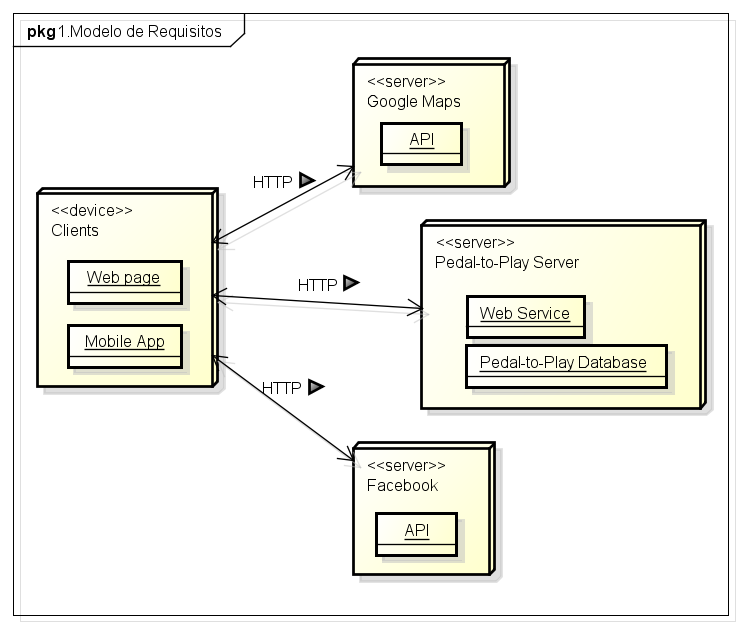
\includegraphics[width=30em]{figuras/arquitetura.png}}
    \label{fig:arquitetura}
\end{figure}

O modelo utilizado na organização dos componentes é o Cliente-Servidor,
no qual os processos de um cliente interagem com os processos de um servidor localizado em um domínio distinto. Os servidores gerenciam e compartilham recursos para seus clientes, podendo também ser clientes de outros servidores \cite{sommerville2003engenharia}.

\par Os clientes do Pedal-to-Play correspondem à aplicação \textit{mobile} e à \textit{web page}, esta última com acesso via navegador Web. Eles poderão requisitar serviços da API do Google Maps para visualização no mapa com as pedaladas monitoradas usando o aplicativo \textit{mobile}, assim como da API do Facebook para compartilhar ações realizadas no sistema. O \textit{web service} próprio do Pedal-to-Play será responsável pela autenticação do usuário e verificação da integridade dos dados enviados para serem salvos no banco de dados, este se localizará na mesma máquina do \textit{web service}.

\par A comunicação entre cliente e servidores utilizará o protocolo de mensagens HTTP e de comunicação TCP/IP. O \textit{web service} do Pedal-to-Play receberá requisições e enviará respostas no formato de arquivo JSON e seguirá a arquitetura REST. Ele não será responsável pelo envio de páginas Web (documentos HTML) ao cliente, as páginas serão dinâmicas e utilizarão requisições AJAX\footnote{Asynchronous Javascript and XML é uma termologia usada para simbolizar o emprego de diferentes tecnologias Web para uma aplicação rapidamente realizar atualizações sem necessidade que baixar a \textit{web page} inteira do servidor, somente requisitando as informações que são variáveis \cite{mdn2015ajax}.} para obtenção dos dados necessários para exibição correta ao usuário. 

\section{Requisitos}
Requisitos podem ser classificados como requisitos funcionais, os quais especificam o que o sistema deve ou não fazer e requisitos não funcionais, que compreendem restrições sobre as funcionalidades do sistema, tais como tempo, processos e padrões\cite{sommerville2003engenharia}. Os requisitos funcionais e não funcionais do Pedal-to-Play serão apresentados a seguir.

\subsection{Requisitos funcionais}
A primeira necessidade é possibilitar o \textbf{Monitoramento da atividade de ciclismo}, o qual deve ser feito através do rastreamento via geolocalização do \textit{smartphone} ou \textit{tablet} do usuário. Após a coleta dos dados da pedalada, o sistema deve calcular a distância do trajeto percorrido, velocidade média e tempo de duração.
\par
A segunda necessidade é o \textbf{Avatar virtual}. O avatar poderá ser customizado de acordo com os desejos do usuário e as peças disponíveis em relação ao nível do mesmo. A visualização do avatar deve estar presente na tela inicial da aplicação.
Ele é composto por dois elementos: o ciclista e a bicicleta. O ciclista é dividido em 3 partes interligadas: cabelo, rosto (olhos, boca e nariz) e equipamentos. Os equipamentos incluem: capacete, \textit{jersey}(malha) e \textit{shorts}, calçados, luva e óculos. Cada nível cumprido torna disponível ao usuário um novo modelo de bicicleta e um novo equipamento. 
\par
A terceira necessidade é a \textbf{Motivação para prática da atividade física}. O Pedal-to-Play deve propor desafios ao usuário, através destes possibilitar a obtenção de recompensas de acordo com os resultados obtidos. As recompensas envolvem novos itens para customizar o avatar. 
\par 
Também para promover motivação, o sistema deve possibilitar o compartilhamento em redes sociais dos feitos dentro da aplicação, tais como o cumprimento de desafios, a inclusão de pedaladas e a customização do avatar. 
\par 
A quarta necessidade é o \textbf{Gerenciamento de usuários}. Esta necessidade envolve a manutenção do cadastro dos usuários; a autenticação deles no sistema e a visualização de informações de desempenho, tais como: nível, distâncias percorridas, velocidade, tempos de atividade e total de distância já percorrida.
\par
A manutenção do cadastro de usuário envolve algumas regras de negócio, tais como:
o email dever ser usado como nome de usuário para autenticação e deverá estar no formato válido de email (\textit{usuario@subdomínio.domínio}); a senha do usuário deve conter de 6 a 30 caracteres e deve ser criptografada logo após a entrada dela no sistema; para o formulário de cadastro ser válido e concluído é necessário que a senha e a senha de confirmação sejam idênticas; os campos de email, senha e confirmação de senha são obrigatórios para cadastro de um novo usuário e não se deve habilitar o registro de um email já cadastrado. 
    
\subsection{Requisitos não funcionais}
O \textit{software} deve utilizar tecnologias do desenvolvimento Web, pois um dos objetivos dele é ser multiplataforma.
\par
O sistema operacional \textit{mobile} suportado deverá ser o Android (a partir da versão 4.1, pois esta é a menor versão disponível para teste nos dispositivos disponíveis e também a que apresenta os requisitos mínimos de todas as tecnologias a serem implementadas). O sistema não terá versão para iOS nativo devido à necessidade de um Apple ID e uma conta de desenvolvedor, a qual para ser mantida ativa é necessário pagar uma anuidade.
\par
Para customização do avatar também é necessário que o dispositivo suporte SVG \textit{inline}\footnote{SVG é um formato de imagens vetoriais baseado em XML\cite{w3c2011svg}}.
\par
Os navegadores suportados para acesso à \textit{web page} deverão ser o Chrome, Firefox e Internet Explorer (a partir da versão 10), pois estes suportam as tecnologias que precisarão ser implementadas no \textit{software}.
\par
A manutenibilidade e portabilidade proporcionada pela implementação de \textit{frameworks}. Tais como, o Bootstrap (versão 3.3.5), para desenvolvimento de \textit{web pages} responsivas e adaptáveis a múltiplos tamanhos de tela; o AngularJS (versão 1.4.6) para o desenvolvimento da parte lógica no cliente usando JS; o Phonegap/Cordova (versão 5.2.0) para compilação do \textit{software} para a plataforma Android e acesso aos recursos de \textit{hardware} dos dispositivos
e o micro \textit{framework} Slim\footnote{\url{http://www.slimframework.com/}} de PHP, o qual é especializado no desenvolvimento de Web APIs e propõe-se a facilitar a implementação das rotas do \textit{web service} (URLs para requisição de recursos do servidor) e gerenciamento de autenticação.
\par
O banco de dados deve ser MySQL e hospedado junto ao servidor, qual deve usar o serviço de hospedagem em nuvem do Red Hat OpenShift. Este serviço possui um plano de uso básico gratuito com uma máquina virtual Linux; suporte a várias linguagens de programação, \textit{frameworks}, banco de dados e servidores Web; integração com Git\footnote{\url{https://git-scm.com/}}; servidores fisicamente localizados na América escalonamento automático da aplicação e acesso SSH.

\pagebreak

\section{Diagrama de Caso de Uso}
Os casos de uso são técnicas de obtenção de requisitos baseadas na representação visual de interações entre componentes de um cenários \cite{sommerville2003engenharia}. O diagrama de Casos de Uso do Pedal-to-Play se encontra na Figura \ref{fig:usecase}.

\begin{figure}[h]
\begin{minipage}{1.0\textwidth}
    \captionof{figure}{Diagrama de Caso de Uso.}
    \centerline{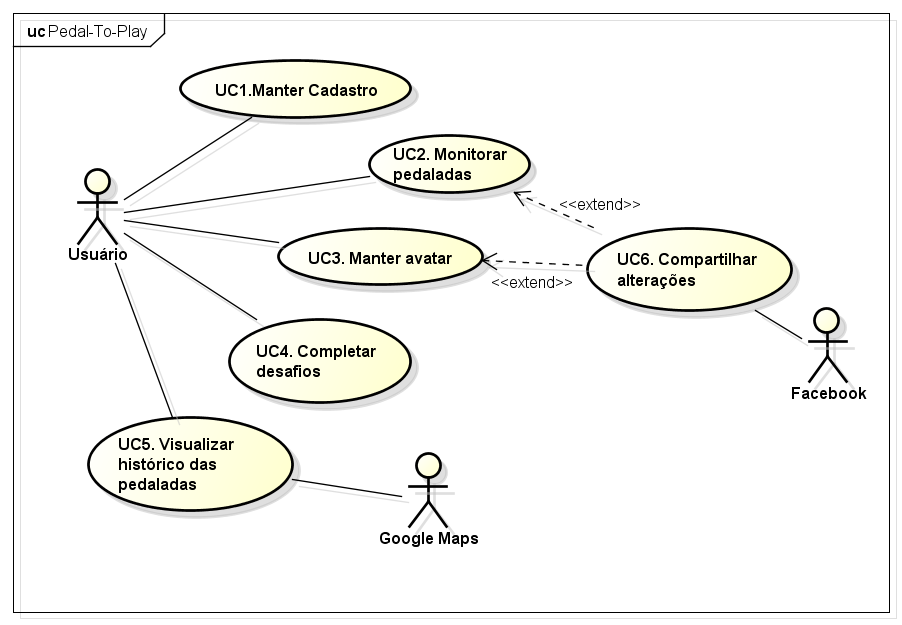
\includegraphics[width=28em]{figuras/useCaseDiagram.png}}
    \label{fig:usecase}
\end{minipage}
\end{figure}

Neste diagrama se encontram seis casos de uso extraídos a partir das necessidades apresentadas nos requisitos funcionais e suas funcionalidades. O caso de uso UC1 está vinculado à necessidade de gerenciamento de usuários; o UC2 à necessidade de monitoramento de atividades; o UC3 à necessidade do avatar e o UC4 e o UC6, à necessidade de motivação. O caso de uso UC5 representa a funcionalidade para visualização das pedaladas monitoradas no Pedal-to-Play e a conexão com a API do Google Maps, o qual é um ator secundário que tem seus serviços requisitados para visualização gráfica dos caminhos das pedaladas. O Facebook também é um ator secundário, o qual pode fornecer seus serviços de compartilhamento de informação. As relações entre o UC6 e os outros casos de uso se classificam como de extensão, pois é uma funcionalidade opcional proposta dentro das funcionalidades de customização do avatar e monitoramento de pedaladas.

\section{Protótipos de telas}
A prototipação de interface gráficas é uma peça fundamental no processo de desenvolvimento de interfaces \cite{sommerville2003engenharia}. Os protótipos de telas do Pedal-to-Play tem o objeto de orientar o desenvolvimento das interfaces gráficas com o usuário (GUI), de modo a detalhar quais elementos devem compô-la, a função de cada um e o posicionamento deles, assim como cores e ícones.  

\subsection{Autenticação de usuário}
Os protótipos da GUI de autenticação compreendem as telas de \textit{login} e cadastro no sistema, as quais podem ser vistas nas Figuras \ref{fig:loginProto} e \ref{fig:signupProto}, respectivamente. Essas GUI tiveram como inspiração as interfaces de autenticação dos aplicativos Strava e Runtastic. 
\par
O botão superior direito em ambas as telas deve permitir a navegação de uma para a outra. O botão inferior deve confirmar os dados preenchidos no formulário e concluir as operações, redirecionando para a tela inicial do sistema em caso dos dados serem aprovados.

\begin{figure}
\centering
\begin{minipage}{.5\textwidth}
  \captionof{figure}{Protótipo da tela\\de login.}
  \centerline{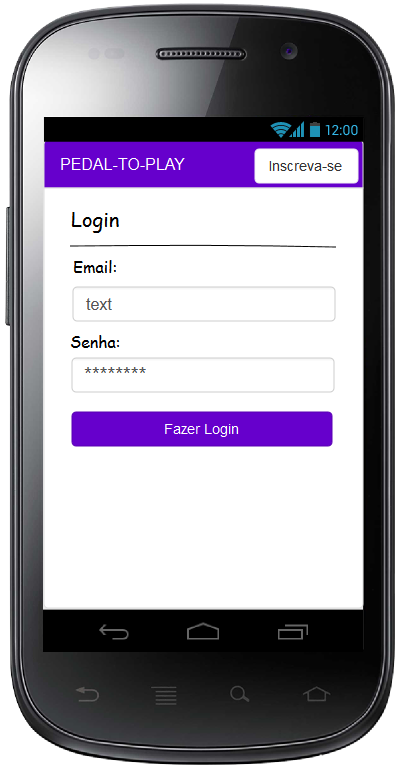
\includegraphics[width=0.7\linewidth]{figuras/Login.png}}
  \label{fig:loginProto}
\end{minipage}%
\begin{minipage}{.5\textwidth}
  \captionof{figure}{Protótipo da tela\\de cadastro.}
  \centerline{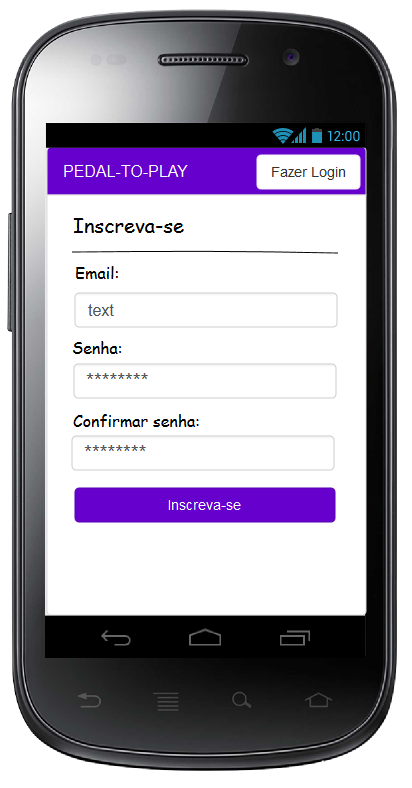
\includegraphics[width=0.7\linewidth]{figuras/Inscreva-se.png}}
  \label{fig:signupProto}
\end{minipage}
\end{figure}

\subsection{Monitoramento de atividade de ciclismo}
Os protótipos do monitoramento de pedalada envolvem as GUI de monitoramento em si (Figura \ref{fig:trackProto}) e a de visualização de pedaladas já monitoradas e registradas no sistema (Figura \ref{fig:recordsProto}). As inspirações para a prototipação dessas interfaces foram, novamente, os aplicativos Strava e Runtastic. 
\par
No protótipo da interface de monitoramento deve haver a opção de gravar a pedalada, a qual deve iniciar o processo de monitoramento via geolocalização do dispositivo \textit{mobile} do usuário. Durante a gravação, as medidas de distância, velocidade e duração devem atualizar-se em tempo real e devem ser exibidas as opções ilustradas na parte direita da Figura \ref{fig:trackProto}. O botão com o ícone de cadeado (botão central dos três inferiores) deve bloquear os outros botões (com o objetivo de evitar toques acidentais), assim desbloqueá-los, permitindo que o usuário possa pausar a gravação ou pará-la. Ao pará-la, o \textit{dialog} para salvar atividade deve ser exibido, nele o usuário pode optar por descartar a gravação ou salvá-la.
\par
O protótipo da interface de visualização do histórico de pedaladas ilustra a visualização dos trajetos de uma pedalada através de um mapa. O histórico de pedaladas remete a lista localizada à direita do mapa. A cima do mapa deve encontrar-se as medidas totais extraídas da pedalada em questão. 

\begin{figure}
\begin{minipage}{1.0\textwidth}
    \captionof{figure}{Protótipo da tela de monitoramento de pedalada.}
    \centerline{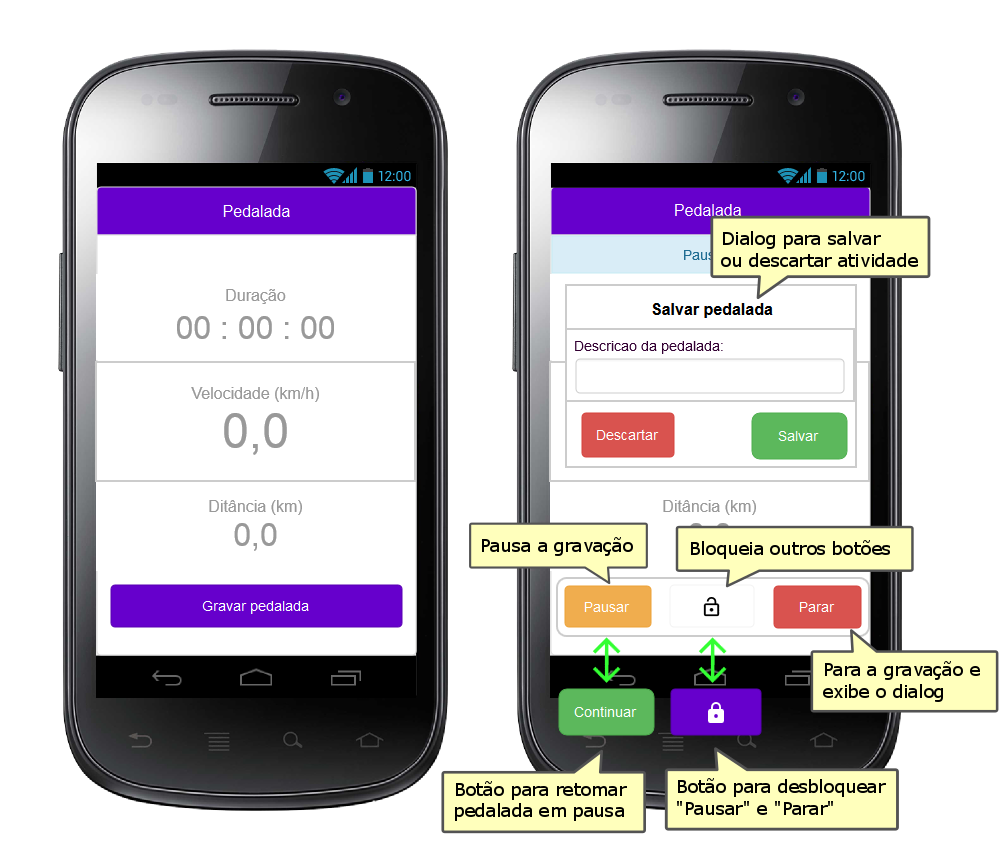
\includegraphics[width=30em]{figuras/Monitoramento.png}}
    \label{fig:trackProto}
\end{minipage}
\end{figure}

\begin{figure}
\begin{minipage}{1.0\textwidth}
    \captionof{figure}{Protótipo da tela de histórico de pedaladas.}
    \centerline{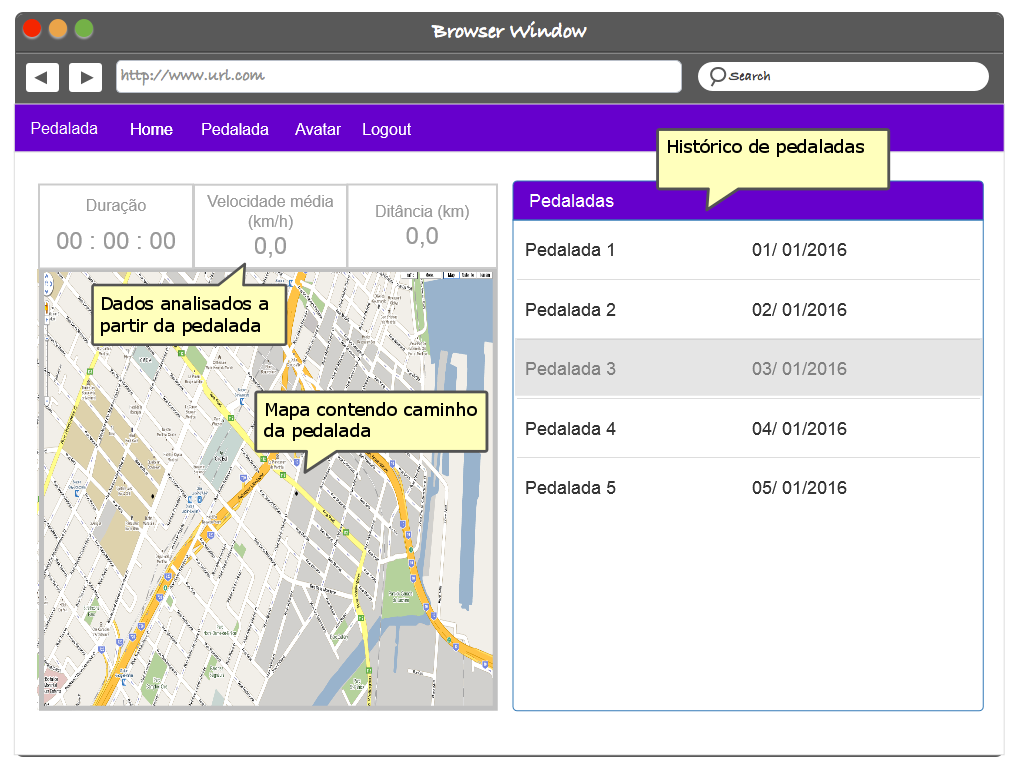
\includegraphics[width=30em]{figuras/Historico.png}}
    \label{fig:recordsProto}
\end{minipage}
\end{figure}

\pagebreak

\subsection{Avatar virtual}
Os protótipos das GUI do sistema do avatar foram inspirados nas interfaces de aplicativos \textit{mobile} existentes no mercado específicos desta temática. Os aplicativos foram escolhidos com base na popularidade deles na Google Play (loja virtual do Google com aplicativos para Android e mídias diversas). Eles são os seguintes: o BuddyPoke\footnote{https://play.google.com/store/apps/details?id=com.buddypoke.buddypoke}; o WeeMee\footnote{https://play.google.com/store/apps/details?id=novoda.weeworld} e o FaceQ\footnote{https://play.google.com/store/apps/details?id=com.miantan.myoface}.
\par
As Figuras \ref{fig:homeProto} e \ref{fig:avatarProto} são os protótipos das interfaces do sistema do avatar virtual, sendo a da esquerda também a tela inicial da aplicação (\textit{Home}).

\begin{figure}[h]
\centering
\begin{minipage}{.5\textwidth}
  \captionof{figure}{Protótipo da tela\\inicial da aplicação.}
  \centerline{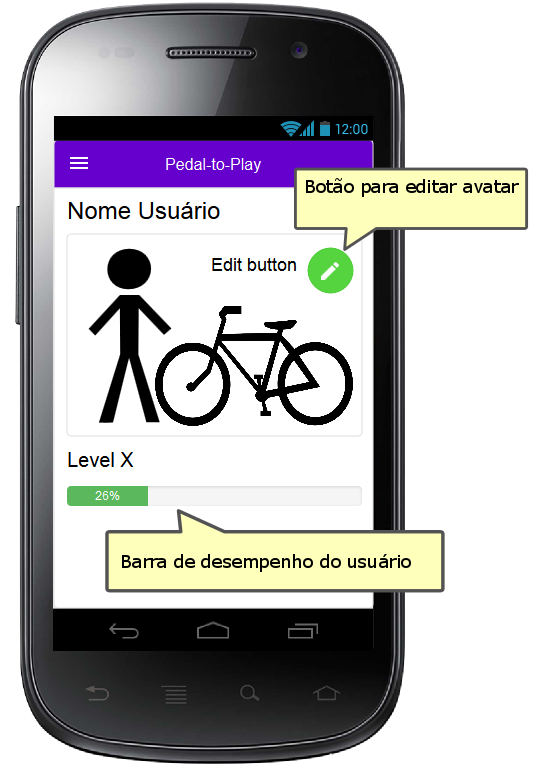
\includegraphics[width=.8\linewidth]{figuras/Visualizacao.png}}
  \label{fig:homeProto}
\end{minipage}%
\begin{minipage}{.5\textwidth}
  \captionof{figure}{Protótipo da tela de\\customização de avatar.}
  \centerline{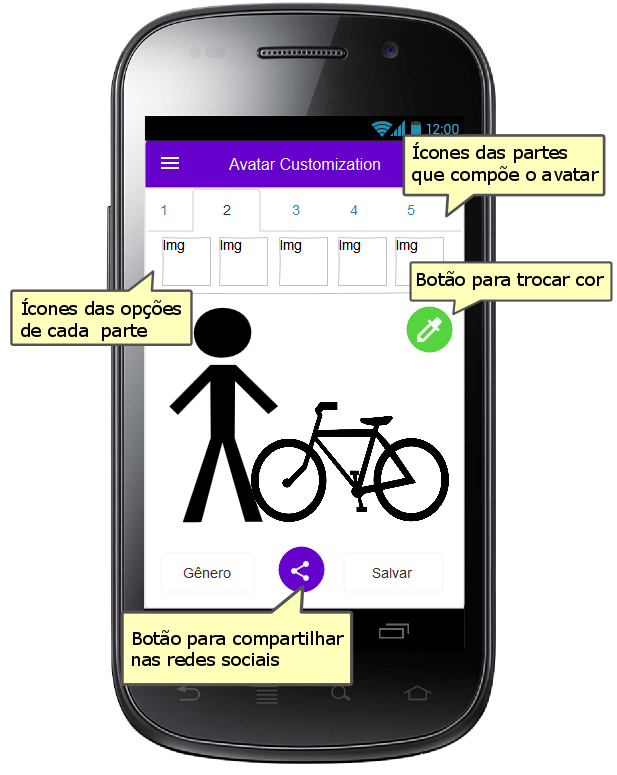
\includegraphics[width=.9\linewidth]{figuras/Customizacao.png}}
  \label{fig:avatarProto}
\end{minipage}
\end{figure}

A tela de \textit{Home} deve possuir, além do avatar, uma barra de progresso que ilustra o desenvolvimento do usuário na atividade de ciclismo, baseado no medida de distância total acumulada. O botão para editar o avatar deve redirecionar para a tela de customização (à direita). A tela de customização do avatar deve ser composta pelos elementos necessários para realizar alterações no avatar, assim como o botão de compartilhamento em redes sociais.

\section{Diagrama de Entidade Relacionamento}
Diagramas de Entidade Relacionamento são utilizados para definir o modo lógico dos dados que serão processados e armazenados pelo sistema. Eles apresentam as entidades que compõe o \textit{software}, seus atributos e o relacionamento entre elas. Esses diagramas servem como base para estruturação e especificação do banco de dados do sistema \cite{sommerville2003engenharia}. A Figura \ref{fig:ermodel} corresponde ao Diagrama de Entidade Relacionamento do Pedal-to-Play.

\begin{figure}
\begin{minipage}{1.0\textwidth}
    \captionof{figure}{Diagrama Entidade Relacionamento.}
    \centerline{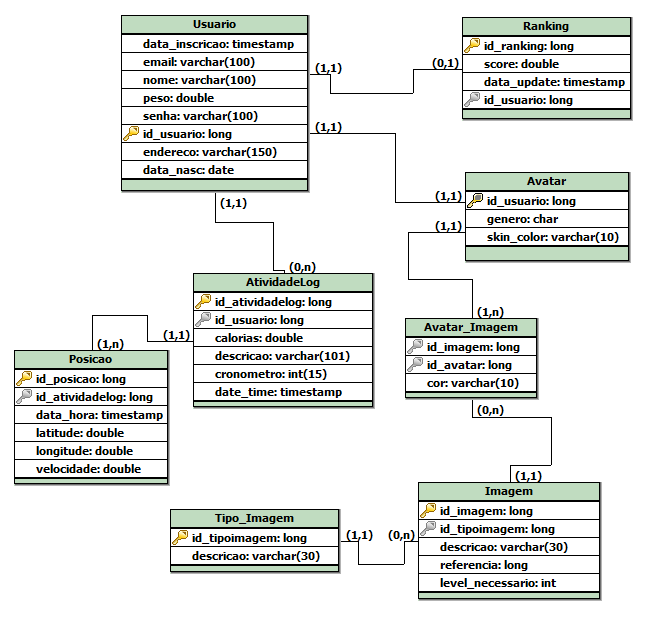
\includegraphics[width=26em]{figuras/er.png}}
    \label{fig:ermodel}
\end{minipage}
\end{figure}

A entidade \textit{User} corresponde ao cadastro de usuário no sistema, ela é o centro do sistema e se relaciona diretamente com as entidades \textit{Ranking}, \textit{Avatar} e \textit{AtividadeLog}. A entidade \textit{Ranking} possui os atributos relacionados à quantificação dos pontos (\textit{score}) de cada usuário, esses pontos determinam o nível em que ele está e são baseados na distância acumulada por todas as pedaladas registradas por ele. O registro de pedaladas e seus dados remetem à entidade \textit{AtividadeLog}, cada registro desta entidade representa uma pedalada e possui relação com vários itens da entidades \textit{Posição}. Cada item da entidade \textit{Posição} refere-se a um elemento retornado pela tecnologia de geolocalização.
\par
A entidade \textit{Avatar} remete aos dados dos avatares virtuais dos usuários. Ela é normalizada nas entidades \textit{Imagem}, a qual se relaciona com a entidade \textit{Tipo\_Imagem} (esta refere-se à categoria do objeto ilustrado na imagem, exemplo: bicicleta, vestimenta ou rosto.) e \textit{Avatar\_Imagem}, sendo esta uma entidade de relacionamento para vincular um avatar e suas várias imagens, assim como uma imagem e os diversos avatares que possam vir a fazer uso dela (tipo de relacionamento \textit{Many-to-Many}).  

\section{Conclusões}
Neste capítulo foram apresentadas as técnicas de análise e projeto do Pedal-to-Play. Incluiu a descrição da arquitetura do sistema, o levantamento de requisitos, a diagramação de casos de uso e de entidade relacionamento, assim como a prototipação de interfaces com o usuário.
\par
No capítulo seguinte será dissertada a implementação dos itens analisados e projetados nas sessões anteriores. O que incluí o Módulo de Autenticação, do Avatar Virtual, de Monitoramento e Registro de Pedaladas e de Desafios.

% ~~~~~~~~~~~~~~~~~~~~~~~~~~~~~~~~~~~~~~~~~~~~~~~~~~~~~~~~~~~~~~~~~~~~~~~~ %

\chapter{Implementação} \label{cap:desenv}
% Introduzir capítulo, falar sobre Implementação.
A etapa de implementação caracteriza-se no processo de projetar os módulos do sistema a partir dos requisitos e arquitetura, adequando estes projetos ao ambiente de desenvolvimento e então, desenvolvendo a solução técnica \cite{openupDevelopment}. 
\par
O processo adotado para desenvolvimento do Pedal-to-Play foi o de Desenvolvimento Incremental, no qual o desenvolvimento do \textit{software} é divido em entregas com prazos curtos, chamadas incrementos, os quais reúnem um conjunto de funcionalidades \cite{sommerville2003engenharia}. Os incrementos do Pedal-to-Play sãos os casos de uso definidos no levantamento de requisitos e cada um deles foi convertido em um módulo do sistema.
\par
Os módulos do Pedal-to-Play estruturam-se no padrão de projeto MVC (Model-View-Controller). Este padrão teve suas origens no Smalltalk e tem como objetivo a separação da apresentação e da lógica do \textit{software} em si. O modelo (Model) corresponde às entidades que compõe o sistema e ao gerenciamento de dados; as visões (Views) referem-se às interfaces do sistema, sejam elas gráficas, linhas de comando ou APIs e os controladores (Controller) são objetos manipuladores das visões e gerenciadores de eventos, os quais atuam como pontes entre o modelo e as visões \cite{burbeck1992applications}. 

\section{Módulo de Autenticação de Usuário}
O módulo de autenticação remete à necessidade de manter um cadastro de usuário e identificá-lo no sistema. Os dados necessários para identificar o usuário são seu email, senha, identificador numérico único (ID) e \textit{token} (sequência de caracteres gerada automaticamente pelo servidor).
\par
A senha do usuário é capturada na GUI de cadastro ou \textit{login} e, ainda no lado do cliente, é criptografada em MD5\footnote{MD5 é um algoritmo de \textit{hashing} que a partir de uma entrada de texto gera uma saída de 128 bits. Presume-se que é computacionalmente inviável produzir uma saída igual para duas mensagens diferentes e descobrir o texto original, tendo somente a saída gerada \cite{rfc1321MD5}} utilizando o módulo de AngularJS, Angular-MD5\footnote{\url{https://github.com/gdi2290/angular-md5}}.
\par
Quando um novo usuário é cadastrado e seus dados são verificados, um \textit{token} e ID são gerados pelo servidor e enviados para o cliente. O \textit{token} e ID são agregados aos cabeçalhos HTTP de todas as requisições feitas pelo cliente para com o servidor, a fim de identificar o usuário que deseja executar alterações em seus dados. Optou-se por usar esta forma de autenticação no lugar da senha e email do usuário para evitar o tráfego excessivo destas informações pela Internet. 
\par
A Figura \ref{fig:authSequence} ilustra como o usuário é autenticado no sistema e identificado em suas requisições ao servidor. E a Figura \ref{fig:authclasses} apresenta o \textit{design} do módulo de autenticação baseado no padrão MVC.

\begin{figure}
\begin{minipage}{1.0\textwidth}
    \captionof{figure}{Processo de autenticação de usuário.}
    \centerline{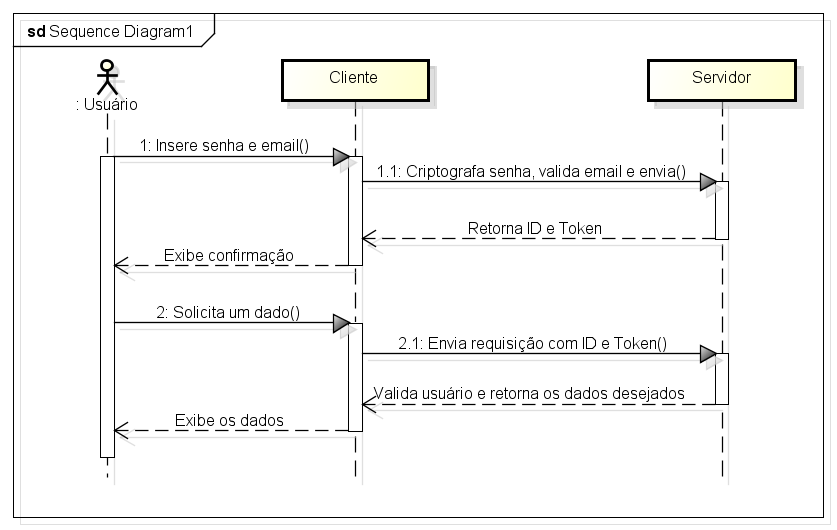
\includegraphics[width=30em]{figuras/authSequence.png}}
    \label{fig:authSequence}
\end{minipage}
\end{figure}

\begin{figure}
\begin{minipage}{1.0\textwidth}
    \captionof{figure}{Diagrama de classes simplificado do Módulo de Autenticação.}
    \centerline{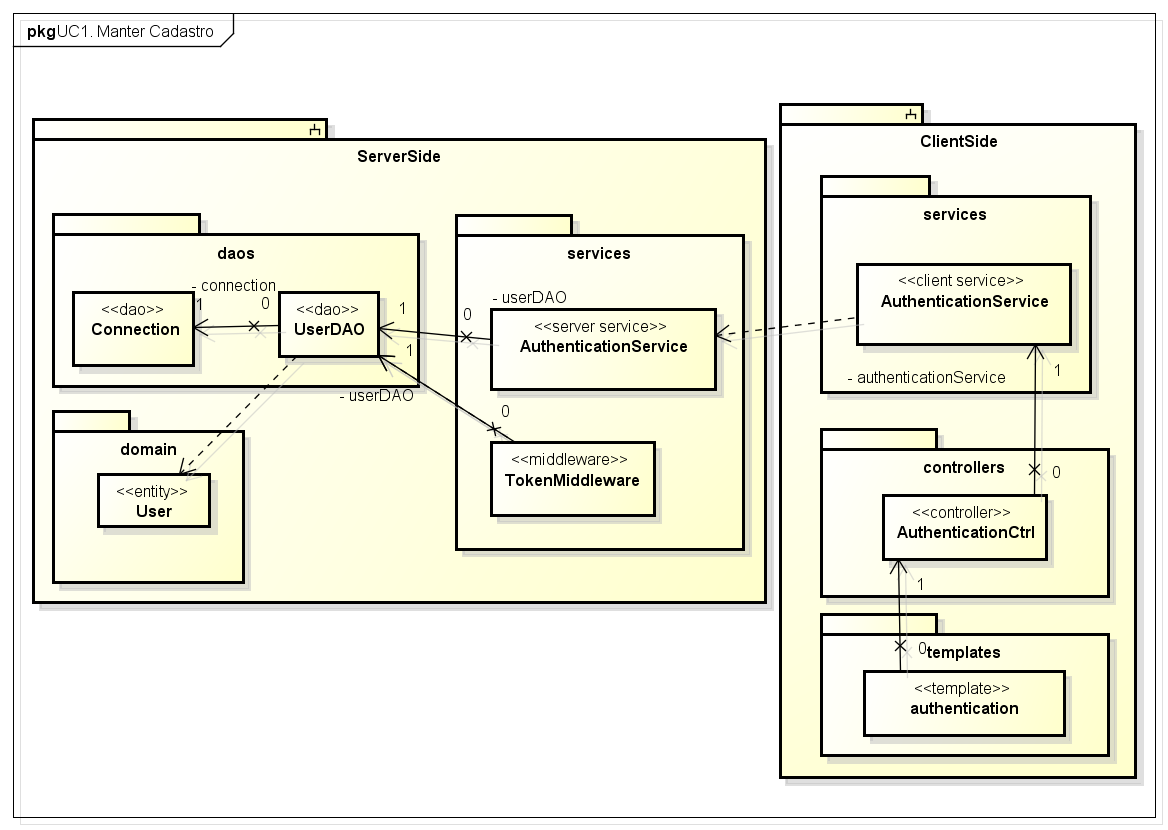
\includegraphics[width=35em]{figuras/authClasses.png}}
    \label{fig:authclasses}
\end{minipage}
\end{figure}

No lado do cliente, os objetos de estereótipo  \textit{template} representam as GUI do sistema e são gerenciados pelos objetos de estereótipo  \textit{controller}. Os \textit{controllers} são responsáveis pelo dinamismo das GUI e, especialmente no módulo de autenticação, a criptografia da senha do usuário. Eles também se comunicam com os objetos de estereótipo  \textit{client service}, cuja responsabilidade é verificar a integridade dos dados de entrada e providenciar o armazenamento ou resgate deles. Os \textit{client service} são a ponte de tráfego de dados entre cliente e servidor. 
\par
O armazenamento de dados no lado do cliente é feito usando o armazenamento local da Web \footnote{\url{http://www.w3.org/TR/webstorage/\#the-localstorage-attribute}}, o acesso a este recurso no Pedal-to-Play é feito pelo módulo de AngularJS, Angular-local-storage\footnote{\url{https://github.com/grevory/angular-local-storage}}.
\par
No lado do servidor, os objetos de estereótipo  \textit{server service} se comportam do mesmo modo dos \textit{client services}, mas além da verificação e tráfego dos dados, os \textit{server services} relacionam-se com os \textit{data access objects} (DAOs). Os DAOs têm a responsabilidade de gerenciar o banco de dados do sistema. Eles se relacionam com os objetos de estereótipo  \textit{domain}, os quais são referências às tabelas do banco de dados.
\par
O objeto \textit{middleware} é um caso especial, sua responsabilidade é validar o cliente que requisitou um serviço do servidor, através do ID e \textit{token} do usuário. \textit{Middleware} é um recurso do \textit{framework} Slim que permite a interceptação de toda requisição ao servidor com o objetivo de fazer uma pré verificação dos dados. No caso do TokenMiddleware, se os dados do usuário forem válidos, a requisição segue seu fluxo normalmente. Do contrário, é disparado um erro para o cliente, com \textit{status} 401 (\textit{Unauthorized})\footnote{\url{http://www.w3.org/Protocols/rfc2616/rfc2616-sec10.html}}.

\section{Módulo de Monitoramento e Registro de Pedaladas}
O módulo de monitoramento compreende dois casos de uso, o monitoramento de uma atividade de ciclismo (usando geolocalização) e a visualização do histórico de atividades passadas. A visualização do histórico pode ser acessada em qualquer dispositivo com a cesso a Internet e um navegador Web (levando em consideração os navegadores suportados pelo sistema), no entanto, o monitoramento é uma função exclusiva dos dispositivos \textit{mobile}, pois utiliza a API do Cordova e seu \textit{plugin} de geolocalização\footnote{\url{https://github.com/apache/cordova-plugin-geolocation}} para acesso ao GPS do dispositivo.
\par
Além do \textit{plugin} de geolocalização, este módulo utiliza os \textit{plugins} do Cordova, Cordova-plugin-network-information\footnote{\url{https://github.com/apache/cordova-plugin-network-information}} e Cordova-diagnostic-plugin\footnote{\url{https://github.com/dpa99c/cordova-diagnostic-plugin}}. Os \textit{plugins}, respectivamente, permitem a verificação do \textit{status} da rede do dispositivo (se este está conectado à Internet e qual o tipo da rede) e permitem verificar se os recursos do dispositivo estão, ou não, ativos (para o monitoramento é importante sabe se o GPS está ativo).
\par
Para desenvolvimento da solução técnica do monitoramento por geolocalização, tomou-se como referência os tutoriais de Brian Ford (desenvolvedor filiado ao Google, envolvido diretamente no projeto do AngularJS)\citeyearpar{fordCordova} e de Mortimer\citeyearpar{mortimer2012}. Ford descreveu como utilizar a plataforma Cordova em conjunto com o \textit{framework} AngularJS e Mortimer descreveu como desenvolver uma aplicação básica para rastrear atividades do usuário usando os recursos de geolocalização do Cordova.
\par
Baseando-se em Ford e Mortimer, o monitoramento de atividades do Pedal-to-Play foi implementado da seguinte maneira: verifica-se a disponibilidade do Cordova, se disponível, verifica-se se o GPS está ativo, se sim, começa o monitoramento. Durante o monitoramento, a GUI se atualiza com os valores retornados da API de geolocalização e exibe para o usuário as opções de Parar e Pausar a atividade. Se o usuário solicitar pausar, pause-se o fluxo até segunda ordem. Se solicitar parar, termina o fluxo e pergunta-se ao usuário se deseja salvar ou descartar a atividade monitorada. Caso a escolha seja salvar, o lado cliente verifica os dados e os envia para o servidor e caso seja descartar, encerra-se o fluxo.
\par
Caso perca-se o sinal do GPS ou aconteçam erros consecutivos na API de geolocalização, pausa-se o monitoramento até que a situação normalize e caso o dispositivo esteja sem conexão com a Internet quando o usuário solicitar o salvamento de uma atividade, a aplicação cliente salva localmente em uma fila. Quando uma atividade é enviada com sucesso ao servidor, a aplicação envia o conteúdo da fila (se está não estiver vazia) em seguida.
\par
No lado do servidor, verificam-se os dados novamente e a autenticação do usuário antes de salvar a atividade. O salvamento se dá pela interpretação da mensagem vinda do cliente, a qual contém as características da atividade (descrição, duração e data) e o trajeto percorrido, composto por um conjunto de objetos \textit{Position}. O objeto \textit{Position} é o retorno da API de geolocalização do Cordova em cada iteração do ciclo de monitoramento. Ele é especificado segundo a W3C e possui os seguintes atributos:
\begin{itemize}
\item \textit{timestamp}: Data e hora do sistema.
\item \textit{coords}: arranjo de coordenadas.
    \begin{itemize}
        \item \textit{latitude}: Latitude em graus decimais.
        \item \textit{longitude}: Longitude em graus decimais.
        \item \textit{altitude}: Altura da posição em metros.
        \item \textit{accuracy}: Nível de precisão da latitude e longitude em metros.
        \item \textit{altitudeAccuracy}: Nível de precisão da altitude em metros. 
        \item \textit{heading}: Direção da viagem, especificado em graus contando no sentido horário em relação ao norte verdadeiro.
        \item \textit{speed}: A velocidade atual do aparelho em relação ao chão, especificado em metros por segundo.
    \end{itemize}
\end{itemize}

\par
A Figura \ref{fig:trackingActivity} ilustra o fluxo principal de monitoramento, desconsiderando possíveis falhas, e a Figura \ref{fig:trackingClasses} apresenta o \textit{design} do módulo de Monitoramento.

\begin{figure}
\begin{minipage}{1.0\textwidth}
    \captionof{figure}{Fluxo principal de Monitoramento de Pedalada.}
    \centerline{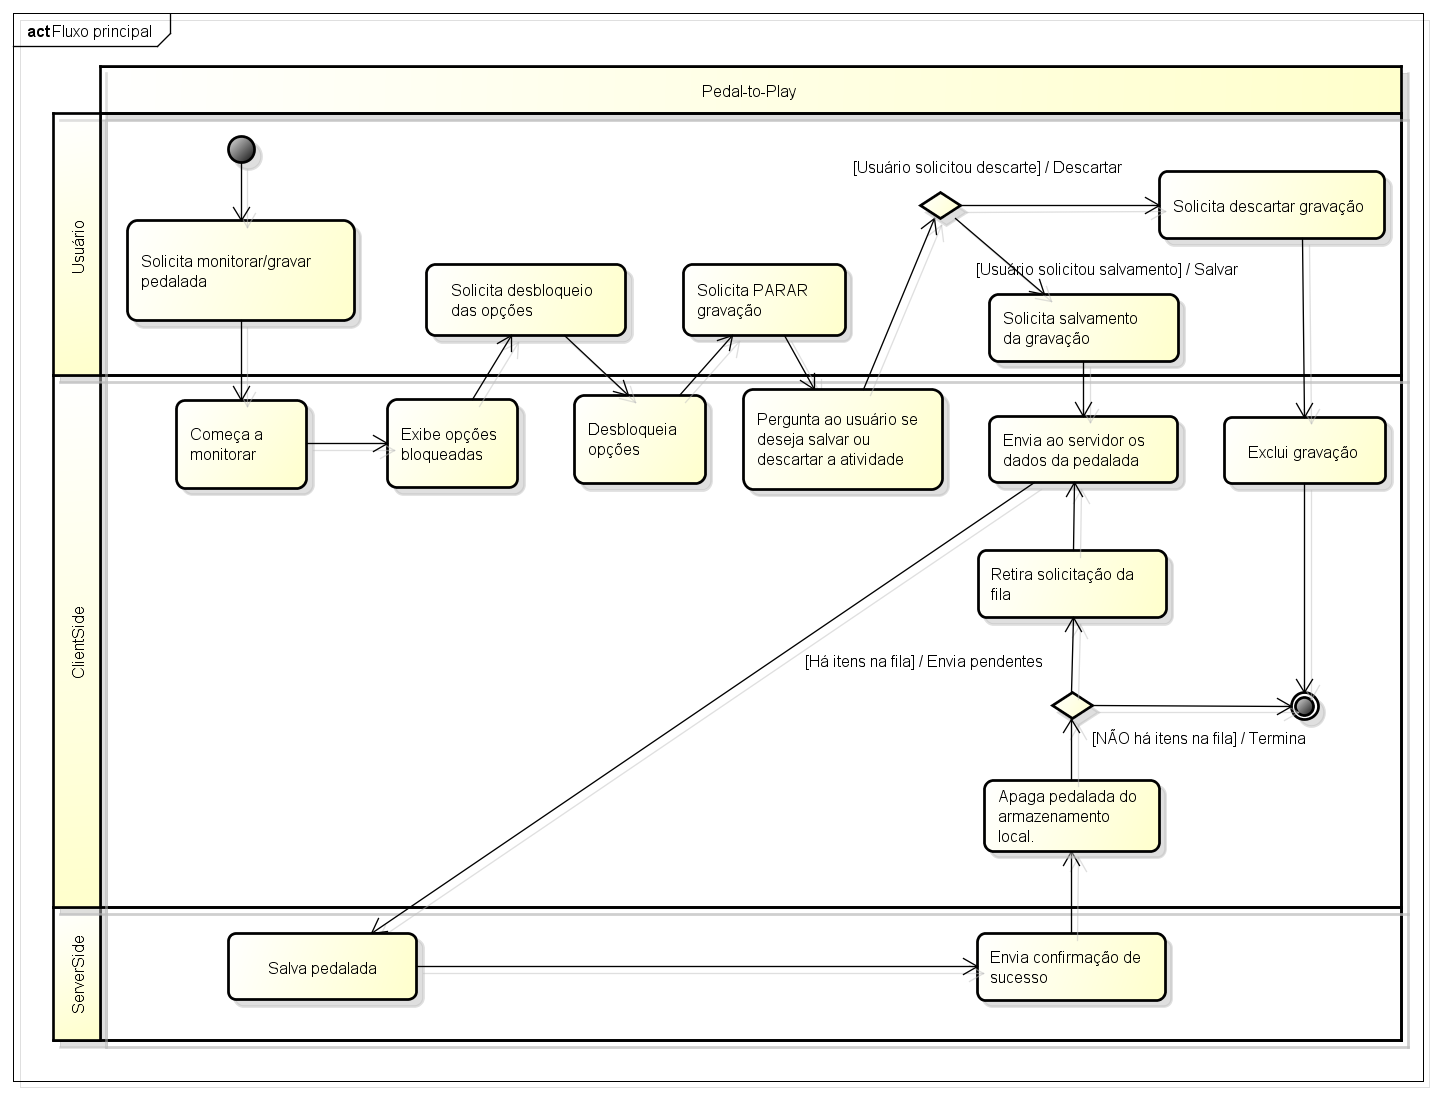
\includegraphics[width=35em]{figuras/trackingActivity.png}}
    \label{fig:trackingActivity}
\end{minipage}
\end{figure}

\begin{figure}
\begin{minipage}{1.0\textwidth}
    \captionof{figure}{Diagrama de classes simplificado do Módulo de Monitoramento de Pedalada.}
    \centerline{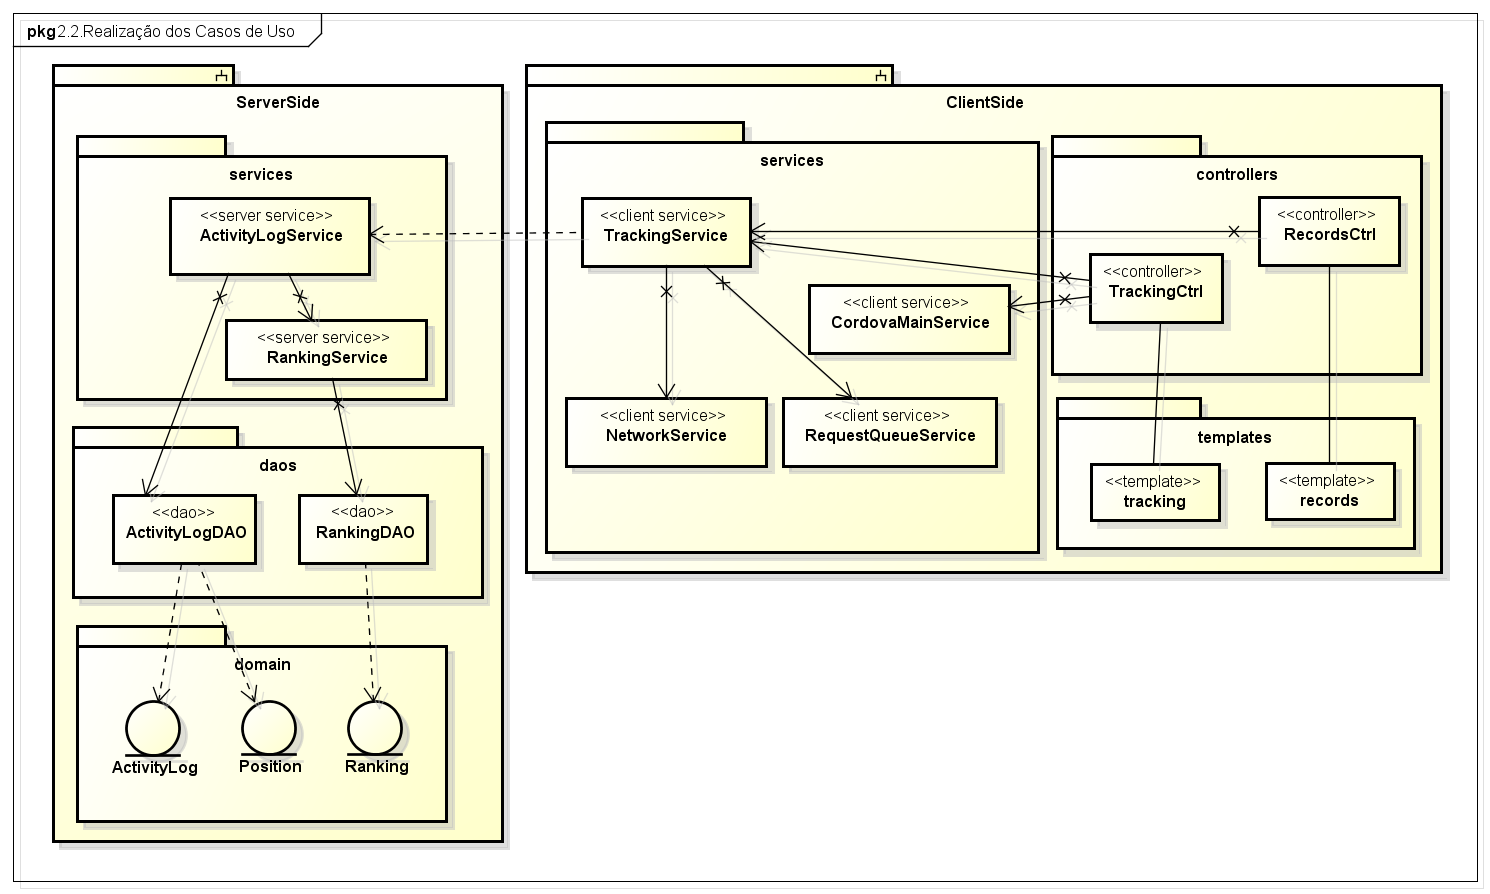
\includegraphics[width=35em]{figuras/trackingClasses.png}}
    \label{fig:trackingClasses}
\end{minipage}
\end{figure}

O objeto \textit{tracking}(\textit{template}) corresponde a GUI de monitoramento e o objeto \textit{records}(\textit{template}), a GUI de visualização do histórico de pedaladas. Eles se relacionam com seus correspondentes \textit{controllers} e estes com os \textit{client services}. O CordovaMainService é responsável pela verificação da disponibilidade da API do Cordova. Caso a API do Cordova não esteja disponível em determinado momento, as requisições feitas a ela são postas em uma fila de espera. Quando a API torna-se disponível, as requisições na fila são invocadas. O RequestQueueService funciona com a mesma lógica, mas com um objetivo diferente, as requisições que ele guarda são as requisições para o servidor. O NetworkService é um \textit{client services} que acessa a API do Cordova para verificar a conexão de rede do dispositivo e o TrackingService é responsável pelo acesso a API de geolocalização, assim como troca de dados com o servidor e funções para verificar a integridade dos dados de uma atividade e analisá-los. A função para determinar a distância do trajeto de uma pedalada se encontra no TrackingService. Ela calcula a distância total do trajeto somando as pequenas distâncias entre todos os pontos que o compõe. O cálculo das pequenas distâncias entre um ponto e outro é baseado no artigo de Veness\citeyearpar{veness2015Distance}. Utiliza-se a seguinte fórmula matemática para obter a distância entre dois pontos de um círculo, chamada de fórmula de Haversine:

\begin{equation}
\begin{split}
a=\sin ^{2}\left( \Delta \varphi  / 2\right) + \cos \varphi 1\cdot \cos \varphi 2\cdot \sin ^{2}\left( \Delta \lambda  / 2\right) 
\\
c=2\cdot{\rm atan2}(\sqrt {a},\sqrt {\left( 1-a\right) })
\\
d=R \cdot c
\end{split}
\label{eqt:calcDistance}
\end{equation}

Na fórmula \ref{eqt:calcDistance}, \varphi \ \  corresponde à latitude; \lambda \ \  à longitude; R ao raio da Terra (6.371km) e d é a distância entre os dois pontos analisados. 
\par
Em relação aos objetos do servidor, o objeto ActivityLogService tem a responsabilidade de interpretar e gerar as mensagens contendo atividades do usuário. Ele se comunica com o ActivityLogDAO, o qual gerencia os dados das atividades no banco de dados. O objeto RankingService tem a responsabilidade de converter a distância percorrida nas atividades para pontos (\textit{score}), os quais determinarão o nível do usuário. Os pontos são armazenados e consultados no banco de dados através do objeto RankingDAO.
\par
Na GUI de \textit{records}, apresenta-se um mapa contendo o trajeto das atividades monitoradas pelo usuário. Ao selecionar uma das atividades presentes no histórico de pedaladas, o cliente requisita ao servidor o conjunto de objetos \textit{Position} referentes àquela atividade e o mapa é renderizado em cima desses dados. Para implementar esse processo, utilizou-se o módulo de AngularJS, Angular Google Maps\footnote{\url{http://angular-ui.github.io/angular-google-maps}}. Este módulo reúne um conjunto de componentes para fácil utilização da API do Google Maps em conjunto com o AngularJS.

\section{Módulo Avatar Virtual}
Para implementação do módulo do avatar virtual, primeiramente foram desenhadas as peças que compõe o personagem. O estilo do avatar foi baseado em ilustrações dos seguintes artistas: Tokyo\footnote{\url{http://opengameart.org/content/anime-style-male-base-sprite}} e Mandi Paugh\footnote{\url{http://opengameart.org/content/anime-style-female-base-sprite}}, do OpenGameArt elythe\footnote{\url{http://elythe.deviantart.com/}}, OrangeNuke\footnote{\url{http://orangenuke.deviantart.com/}}, Dlite-Yamato\footnote{\url{http://dlite-yamamoto.deviantart.com/}} e Pencil-Fluke\footnote{\url{http://pencil-fluke.deviantart.com/}}, do DevianArt. As bicicletas foram desenhadas com base nos modelos disponíveis no \textit{web site} da Century Cycles\footnote{\url{http://centurycycles.com/}} e os equipamentos, nos disponíveis no \textit{web site} da Cycle Ronda\footnote{\url{http://www.cycleronda.com/}}.
\par
Após os desenhos, iniciou-se o desenvolvimento da solução técnica. Todos os desenhos foram feitos no formato SVG e para a manipulação deles via programação, utilizou-se a biblioteca de JS, Snap.svg\footnote{\url{http://snapsvg.io/}}, específica para manipulação de SVG.
\par
A API do Snap.svg possibilitou o mecanismo de customização do avatar, operando da seguinte forma: uma combinação padrão de peças é carregada inicialmente para o DOM da interface de customização. A partir desta combinação inicial, o usuário pode customizar o avatar à vontade, selecionando as peças desejadas que estejam disponíveis para o seu nível. Cada troca de peça remove a parte selecionada do DOM e inclui a nova parte, retirada dos arquivos SVG, os quais contêm todas as peças desenhadas. O número de opções de equipamentos e bicicletas é limitado no nível inicial, mas as opções aumentam conforme o usuário cumpra os desafios e eleve o seu nível.
\par
O usuário também tem a liberdade de definir a cor de pele do personagem e o gênero do mesmo. Para a seleção de cor, utilizou-se o \textit{plugin} de Bootstrap, Bootstrap-Colorpicker\footnote{\url{http://mjolnic.com/bootstrap-colorpicker/}}. Ele proporciona um componente de paleta de cores para a seleção, com estilo Bootstrap e uma API de JS baseada em jQuery, para controle sobre os eventos de seleção de cor.
\par
O armazenamento da customização do Avatar é realizado localmente e no servidor. Para enviar os dados do avatar do cliente para o servidor, utilizou-se uma requisição HTTP para o \textit{web service}, trafegando uma mensagem no formato JSON. Esta mensagem contém os identificadores de cada peça que compõe o avatar, assim como a cor de pele e o gênero do personagem. O diagrama de classes simplificado do módulo avatar está ilustrado na Figura \ref{fig:avatarClasses}. 
% Explicar cada diagrama
\begin{figure}[h]
\begin{minipage}{1.0\textwidth}
    \captionof{figure}{Diagrama de classes simplificado do Módulo do Avatar.}
    \centerline{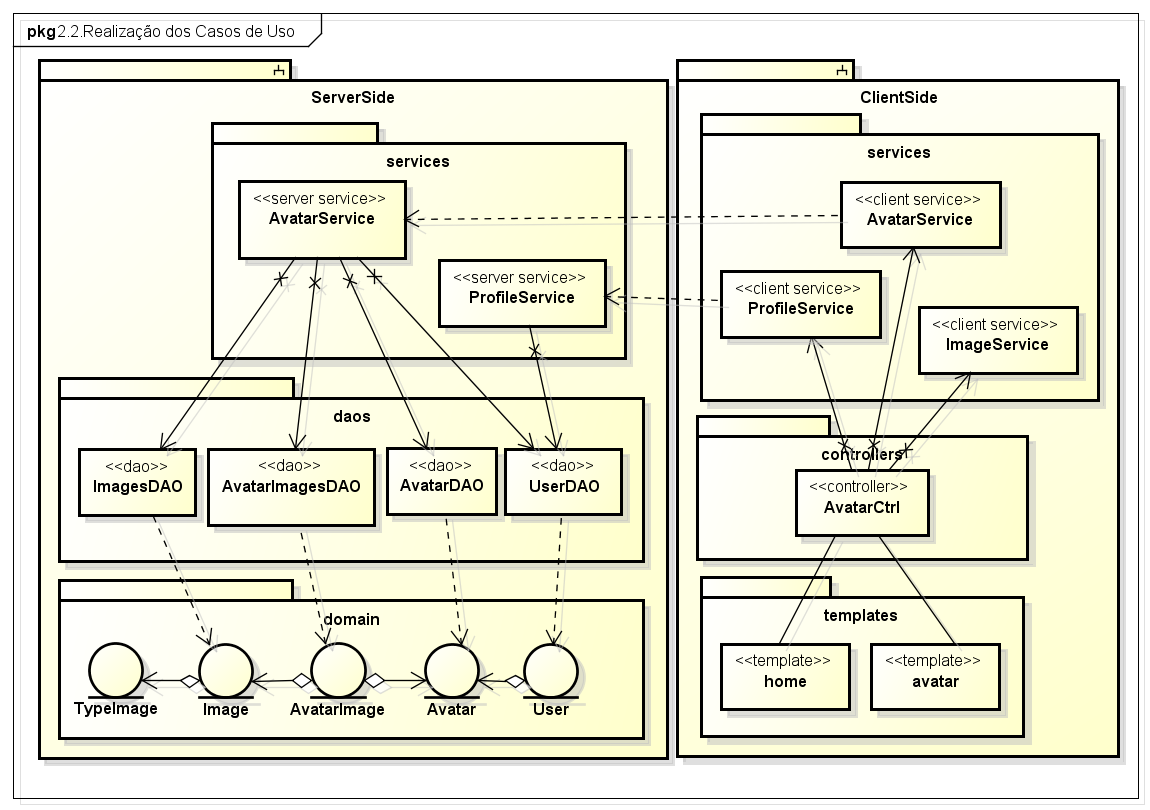
\includegraphics[width=33em]{figuras/avatarClasses.png}}
    \label{fig:avatarClasses}
\end{minipage}
\end{figure}

No lado do cliente, o objeto AvatarCtrl é responsável pela manipulação das imagens do avatar e dos eventos provindos da interação do usuário com a GUI. O AvatarService é responsável pela troca de dados com o servidor; o ImageService, pelo resgate das imagens do sistema de arquivos local para a aplicação e o ProfileService, pela troca de dados relativos ao usuário, entre eles, o nível, que define quais peças do avatar estarão disponíveis para customização. A visualização do avatar (sem opções de customização) é localizada na tela inicial do sistema.
\par
No lado do servidor, os objetos \textit{server services} interpretam os dados enviados pelo cliente, garantem a integridade desses dados e os encaminham para os DAOs, os quais salvam cada peça do avatar em seu devido local no banco de dados. 

\section{Módulo de Desafios}
O módulo de desafios contemplará uma série de tarefas propostas ao usuário que, quando cumpridas, o recompensam com itens para customizar o avatar. Em primeiro momento, haverá quatro desafios, cada um disponível para um nível. Quando os desafios de um nível são completados, o nível do usuário aumenta em um.
\par
Para a elaboração dos desafios foram pesquisados modelos de treinamento de ciclismo, o livro "The Cyclist's Training Bible" de Joe Friel\citeyearpar{friel2012cyclist} possui uma coletânea de planos e técnicas de ciclismo, baseados no tempo de atividade, cadência e potência. No entanto, a cadência e potência necessitam de equipamentos específicos para serem medidas e o tempo não garante que o usuário estava em movimento durante o monitoramento da atividade. Por estes motivos, decidiu-se utilizar a variável \textbf{distância} como requisito nos desafios.
\par
A quantidade de distância para cumprir o primeiro desafio baseou-se em um dos principais segmentos de ciclismo da cidade de Porto Alegre, o trajeto Ipiranga-Hipódromo, disponível no aplicativo Strava (Figura \ref{fig:segment}). Este trajeto tem 5.7km.

\begin{figure}[h]
\begin{minipage}{1.0\textwidth}
    \captionof{figure}{Ipiranga-Hipódromo: Segmento de pedalada em Porto Alegre, Rio Grande do Sul, Brazil.}
    \centerline{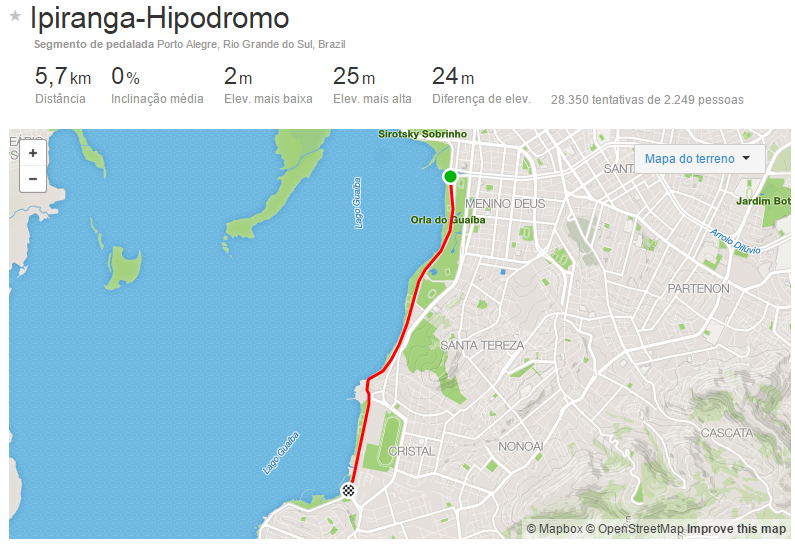
\includegraphics[width=25em]{figuras/stravaSegment.png}}
    \label{fig:segment}
\end{minipage}
\centerline{Fonte: \textit{Print screen} da aplicação Strava.}
\end{figure}

Cada desafio aumenta exponencialmente a quantidade de distância necessária. O desafio de nível 1, para ser cumprido, necessita de pelo menos uma pedalada em um percurso com distância equivalente a do seguimento Ipiranga-Hipódromo; o de nível 2, quatro pedaladas; de nível 3, 10 pedalas e de nível 4, 20 pedaladas, este é o último desafio pois o nível 5 é o último. Os desafios estão descritos na tabela \ref{tab:quests}, assim como suas recompensas e níveis necessários.

\begin{table}
\centering
\caption{Desafios propostos nos níveis do Pedal-to-Play}
\label{my-label}
\begin{tabular}{ccc}
\rowcolor[HTML]{C0C0C0} 
\multicolumn{1}{c|}{\cellcolor[HTML]{C0C0C0}{\color[HTML]{FFFFFF} \textbf{Nível}}} & \multicolumn{1}{c|}{\cellcolor[HTML]{C0C0C0}{\color[HTML]{FFFFFF} \textbf{Requisitos do Desafio}}} & {\color[HTML]{FFFFFF} \textbf{Recompensas}} \\ \hline
\multicolumn{1}{c|}{1}                                                             & \multicolumn{1}{c|}{Acumular 5 km de pedalada.}                                                    & Luvas e BMX.                                 \\ \hline
\multicolumn{1}{c|}{2}                                                             & \multicolumn{1}{c|}{Acumular 20 km de pedalada.}                                                   & Sapatos e Mountain.                       \\ \hline
\multicolumn{1}{c|}{3}                                                            & \multicolumn{1}{c|}{Acumular 50 km de pedalada.}                                                   & Óculos e Road bike.                           \\ \hline
\multicolumn{1}{c|}{4}                                                             & \multicolumn{1}{c|}{Acumular 100 km de pedalada.}                                                  & Vestimenta e Triathlon bike.                 \\ \hline
\end{tabular}
\label{tab:quests}
\end{table}

\section{Compilação para Mobile e Hospedagem do Web Service}
Outras atividades que demandaram um tempo considerável da implementação foram a adequação do projeto para a plataforma Android (usando Cordova) e a hospedagem do \textit{web service}.
\par
Para compilação do projeto em uma aplicação \textit{mobile} foram analisados os \textit{frameworks} Ionic\footnote{\url{http://ionicframework.com/}} e Phonegap\footnote{\url{http://phonegap.com/}}. Ambos são construídos em cima da plataforma Cordova. O Phonegap foi a primeira distribuição do Cordova, enquanto o Ionic é uma distribuição mais recente. O diferencial do Ionic é o uso em conjunto do \textit{framework} AngularJS. Devido a esta característica, foi cogitado utilizar o Ionic para desenvolvimento da versão \textit{mobile} do Pedal-to-Play, pois o lado cliente do sistema é baseado em AngularJS. Todavia, o Ionic, além de um \textit{framework} Cordova, também é um \textit{framework} de CSS. Ele possui estilos próprios para desenvolvimento da GUI e estes estilos não eram interessantes para o Pedal-to-Play, pois são específicos para \textit{mobile} e não se ajustam corretamente em telas grandes, como a de um computador pessoal. Sendo um dos objetivos deste projeto ser multiplataforma, essa característica do Ionic tornaria-se uma desvantagem. Então, optou-se por utilizar o Phonegap e o Bootstrap para os estilos da GUI, o qual tem boa responsividade para qualquer tamanho de tela. 
\par
Em conjunto com o Bootstrap, utilizou-se o \textit{plugin} Jasny-Bootstrap\footnote{\url{http://www.jasny.net/bootstrap/}}, para criação do menu de navegação lateral entre as telas do sistema. Este menu aparece somente em telas com largura menor que 768 \textit{pixels}. 
\par
Para captura de eventos \textit{touch sreen} nos dispositivos \textit{mobile}, o Pedal-to-Play também agregou o módulo de AngularJS, ngTouch\footnote{\url{https://docs.angularjs.org/api/ngTouch}}. E para iconografia, a biblioteca Font Awesome\footnote{\url{https://fortawesome.github.io/Font-Awesome/}} 
\par
Em relação à hospedagem do \textit{web service}, foi necessário conFigurar o servidor para suportar requisições de domínio cruzado (CORS) e um aprofundamento no \textit{framework} Slim. Para conFiguração do CORS utilizou-se o tutorial de Remy Shrap \citeyearpar{remyCors} e o tutorial do Apache sobre o arquivo “.htaccess” \citeyearpar{htaccess}.
\par
O \textit{web service} foi hospedado em um plano gratuito na plataforma Openshift. Também foi cogitado o uso do serviço do Hostinger. No entanto, as características do Openshift mostraram-se mais interessantes, entre elas: servidor com máquina virtual Linux; suporte a várias linguagens de programação, \textit{frameworks}, banco de dados e servidores Web; integração com Git; servidores fisicamente localizados na América escalonamento automático da aplicação e acesso SSH.

\section{Softwares Terceiros Utilizados}
Além dos módulos de AngularJS, dos \textit{plugins} de Cordova e de Bootstrap citados anteriormente, o Pedal-to-Play também fez uso dos seguintes softwares de terceiros para o desenvolvimento da solução técnica:

\begin{itemize}
\item UI Router: módulo de AngularJS para gerenciamento das URLs e transições entre as páginas Web do sistema\footnote{\url{http://angular-ui.github.io/ui-router/site/\#/api/ui.router}}; 
\item Gap Debug: ferramenta para \textit{debug} de aplicações desenvolvidas em Phonegap diretamente nos dispositivos \textit{mobile}\footnote{\url{https://www.genuitec.com/products/gapdebug/}};
\item Visual Studio Code: editor de texto da Microsoft com vários recursos para desenvolvimento de aplicações em JS\footnote{\url{https://code.visualstudio.com/}};
\item Netbeans IDE: ambiente de desenvolvimento com suporte a várias linguagens. Utilizou-se este \textit{software} para desenvolvimento do \textit{web service}\footnote{\url{https://netbeans.org/}};
\item Firefox Developer Edition: navegador baseado no Mozilla Firefox com recursos auxiliares para desenvolvimento de aplicações Web\footnote{\url{https://www.mozilla.org/pt-BR/firefox/developer/}}.
\end{itemize}

\section{Conclusões}
Neste capítulo foi apresentado como decorreu a implementação dos módulos de Autenticação, Avatar, Monitoramento de pedaladas e Desafios. Assim como o resumo de atividades e recursos que envolveram o desenvolvimento destes módulos, tais como a compilação do projeto para Mobile, a hospedagem do servidor e os \textit{softwares} terceiros agregados ao projeto ou que serviram de apoio ao desenvolvimento dele.
\par
O módulo de integração com redes sociais não foi desenvolvido, embora constasse no planejamento do projeto. O calendário planejado era utópico comparado ao tempo que foi necessário de fato para o desenvolvimento de cada módulo. O gráfico presente na Figura \ref{fig:gantt} ilustra a fase de implementação e apresenta quanto tempo utilizou-se para desenvolvimento de cada módulo e atividades relacionadas, totalizando 99 dias.

\begin{figure}[h]
\begin{minipage}{1.0\textwidth}
    \captionof{figure}{Gráfico de Gantt referente ao período de implementação.}
    \centerline{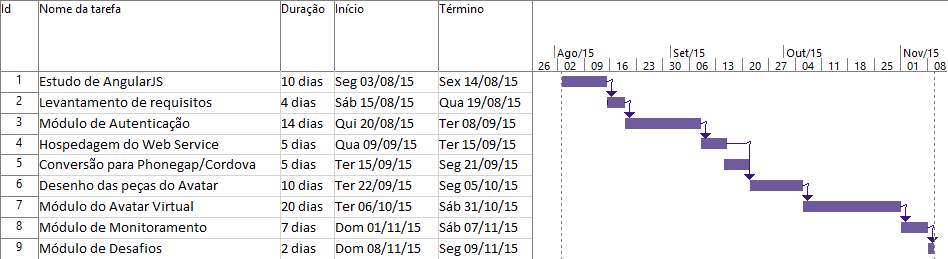
\includegraphics[width=35em]{figuras/ganttDesenv.png}}
    \label{fig:gantt}
\end{minipage}
\end{figure}

%A arquitetura final do sistema, após a fase de implementação, está %representada na \ref{fig:arquiteturaFinal}.
%
%\begin{figure}
%\begin{minipage}{1.0\textwidth}
%    \captionof{figure}{Arquitetura final do sistema.}
%    \centerline{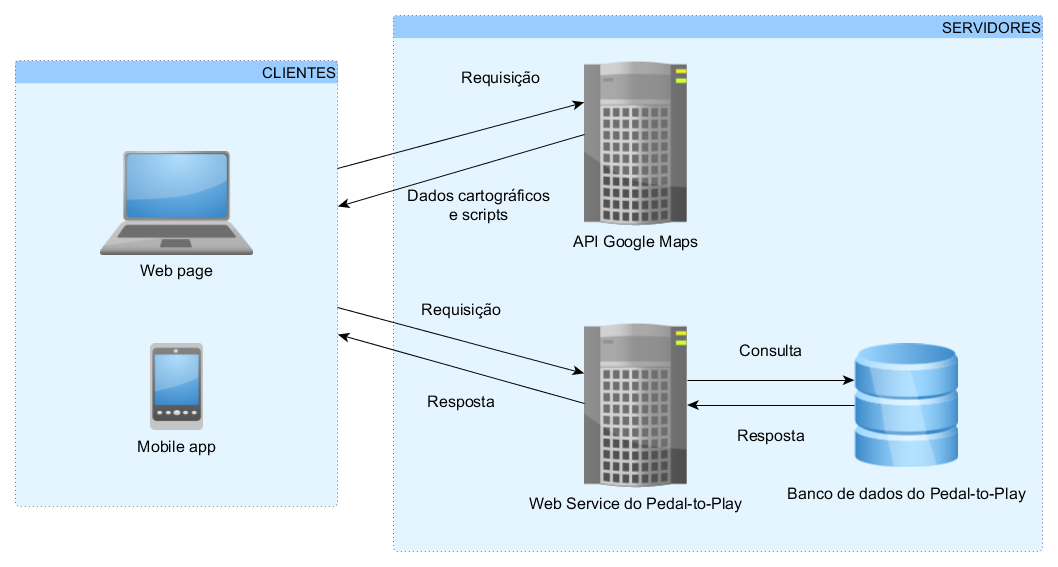
\includegraphics[width=30em]{figuras/arquiteturaFinal.png}}
%    \label{fig:arquiteturaFinal}
%\end{minipage}
%\end{figure}

O próximo capítulo apresentará os resultados obtidos a partir dos módulos implementados. Incluindo \textit{print screens} do sistema e a descrição dos testes de monitoramento de pedaladas reais.

% Cronograma
%%Arquivo contendo o capítulo Cronograma
\chapter{Cronograma} \label{cap:cronograma}
As atividades serão desenvolvidas conforme o cronograma mostrado na Tabela \ref{cronograma}.

\begin{table}[h]
\caption{Cronograma de atividades}
\begin{center}
\begin{tabular}{l|c|c|c|c}
\hline
\multirow{2}{*}{Tarefa} & 
\multicolumn{4}{c}{2015}\\& Ago & Set & Out & Nov 
    \\ \hline
    Levantamento de Requisitos  
        & x   & ~   & ~   & ~    
    \\ \hline
    Prototipação das Interfaces com Usuário
        & x   & ~   & ~   & ~  
    \\ \hline
    Desenvolvimento do \textit{Template} do Sistema
        & x   & ~   & ~   & ~      
    \\ \hline
    Análise do Sistema
        & x   & ~   & ~   & ~
    \\ \hline
    Desenvolvimento do Módulo de Rastreamento de Atividades 
        & ~   & x   & ~   & ~
    \\ \hline
    Desenvolvimento do Lado do Servidor                                 
        & ~   & x   & ~   & ~
    \\ \hline
    Desenvolvimento do Módulo Avatar                        
        & ~   & x   & ~   & ~
    \\ \hline
    Desenvolvimento Módulo Perfil do Usuário
        & ~   & ~   & x   & ~
    \\ \hline
    Desenvolvimento Módulo de Desafios
        & ~   & ~   & x  & ~
    \\ \hline
    Desenvolvimento da Integração com Redes Sociais         
        & ~   & ~   & x  & ~
    \\ \hline
    Finalização dos Testes                                     
        & ~   & ~   & ~  & x
    \\ \hline
    Finalização da Monografia                               
        & ~   & ~   & ~  & x
    \\ \hline
\end{tabular}
\end{center}
\label{cronograma}
\end{table}

% Resultados
\chapter{Resultados}  \label{cap:resultados}
Este capítulo apresentará os resultados obtidos após a fase de implementação. Inclui a apresentação das funcionalidades do sistema por \textit{print screens} e a descrição dos testes realizados monitorando pedaladas reais.

\section{Apresentação das Funcionalidades do Sistema}
A Figura \ref{fig:printLogin} é um \textit{print screen} do formulário de \textit{login} e a Figura \ref{fig:printHome}, da tela inicial da aplicação, para qual o usuário é redirecionado após o \textit{login} ser realizado com sucesso.

\begin{figure}[h]
\begin{minipage}{.5\textwidth}
    \centering
    \captionof{figure}{GUI de \textit{login}.}
    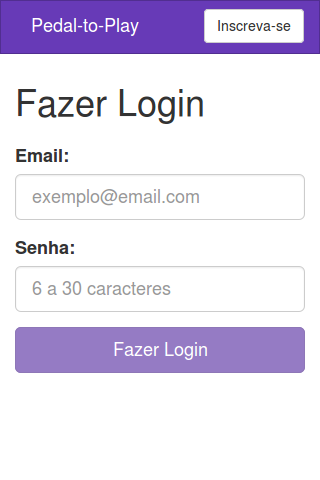
\includegraphics[width=.47\linewidth]{figuras/p2pAuth.png}
    \label{fig:printLogin}
\end{minipage}%
\begin{minipage}{.5\textwidth}
    \centering
    \captionof{figure}{GUI inicial do Pedal-to-Play.}
    \centerline{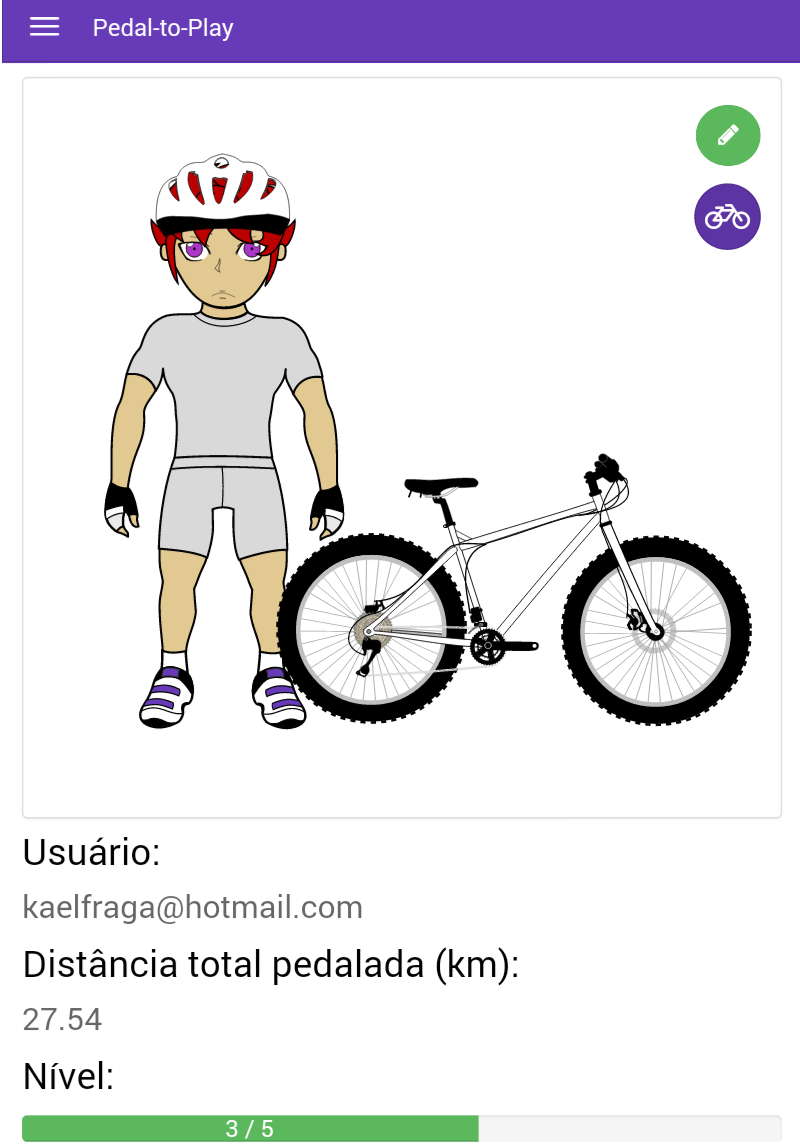
\includegraphics[width=.5\linewidth]{figuras/p2pHome.png}}
    \label{fig:printHome}
\end{minipage}
\par%
\bigskip
\centerline{Fonte: \textit{Print screens} do Pedal-to-Play.}
\end{figure}

Além dos itens especificados na prototipação, a GUI inicial do sistema apresenta os itens "Distância total pedalada" e o botão com ícone de bicicleta. O primeiro informa a soma dos quilômetros percorridos pelo usuário em todas as atividades já monitoradas e o segundo redireciona para a GUI de monitoramento (ou para a GUI de histórico de pedaladas, se o usuário está acessando o sistema via \textit{web page}). Outro detalhe é a informação contida na barra de progresso, correspondente ao nível atual do usuário em relação à quantidade de níveis existentes. 
\par
As Figuras \ref{fig:avatarMobile} e \ref{fig:avatarWeb} correspondem à funcionalidade de customização do avatar virtual respectivamente, para dispositivos com pouca largura de tela (tais como os \textit{smartphones}) e para dispositivos com telas largas (\textit{tablets} e \textit{desktops}).   

\begin{figure}
\begin{minipage}{.4\textwidth}
    \centering
    \captionof{figure}{GUI de customização\\para telas pequenas.}
    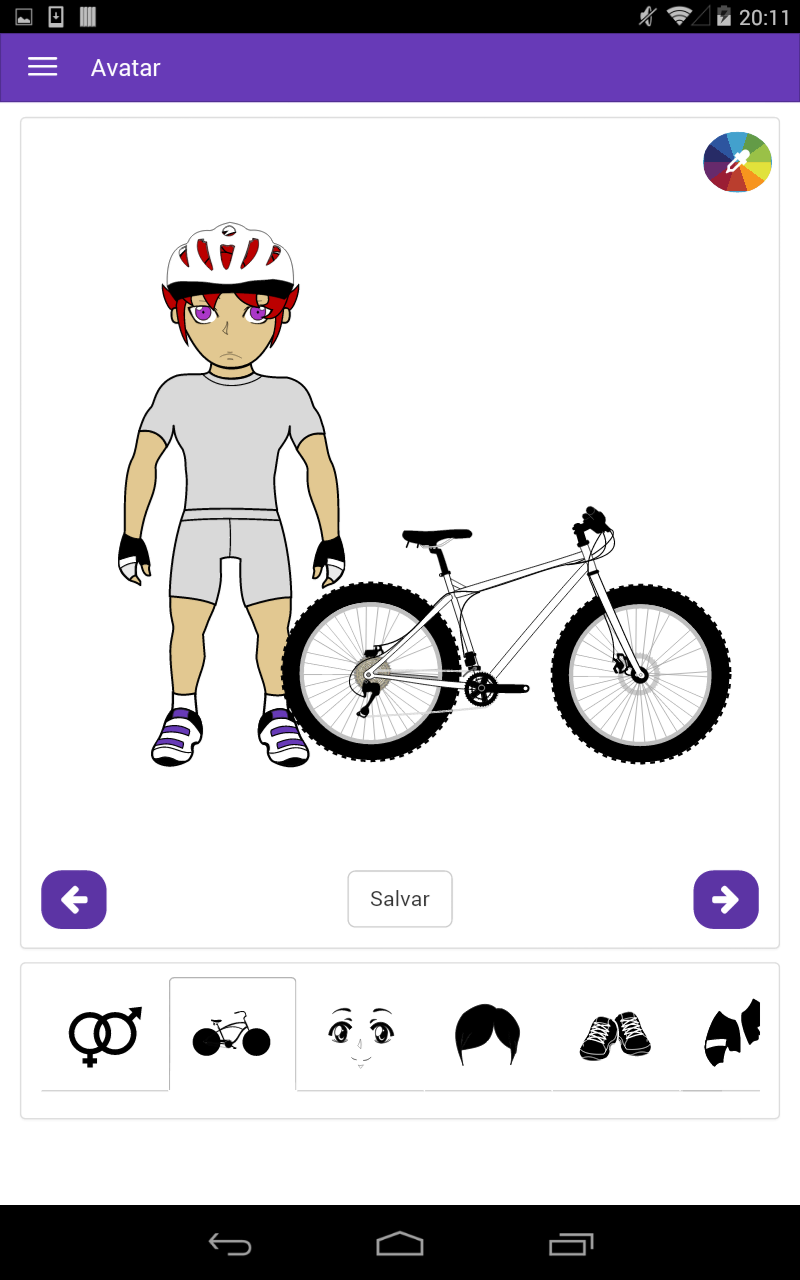
\includegraphics[width=.6\linewidth]{figuras/p2pAvatar.png}
    \label{fig:avatarMobile}
\end{minipage}%
\begin{minipage}{.6\textwidth}
    \centering
    \captionof{figure}{GUI de customização\\para telas grandes.}
    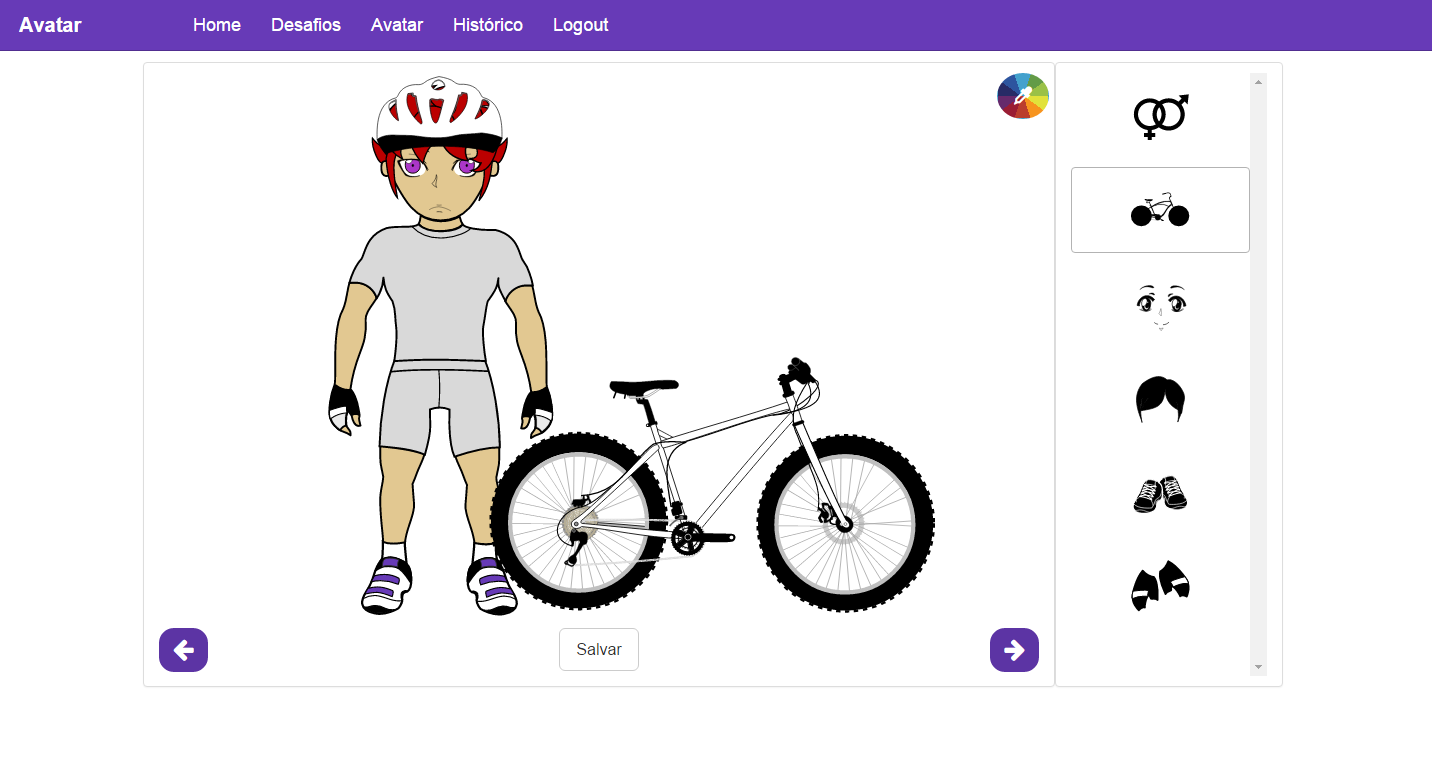
\includegraphics[width=1.1\linewidth]{figuras/p2pWebAvatar.png}
    \label{fig:avatarWeb}
\end{minipage}
\par%
\bigskip
\centerline{Fonte: \textit{Print screens} do Pedal-to-Play.}
\end{figure}

Diferente dos protótipos, a mudança de peças do avatar é realizada selecionando uma categoria de peça entre as disponíveis e usando os botões direcionais para navegar entre as opções de cada categoria.
\par
A Figura \ref{fig:trackingMobile} apresenta a funcionalidade de monitoramento de pedalada em execução, mostrando a velocidade atual do usuário, a distância total percorrida e o tempo total da atividade corrente até o momento do \textit{print screen}.

\begin{figure}[h]
\begin{minipage}{1.0\textwidth}
    \captionof{figure}{Monitoramento de pedalada em execução.}
    \centerline{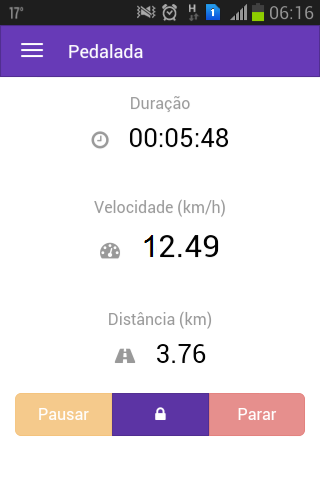
\includegraphics[width=10em]{figuras/p2pTracking.png}}
    \label{fig:trackingMobile}
\end{minipage}
\centerline{Fonte: \textit{Print screen} do Pedal-to-Play.}
\end{figure}

As Figuras \ref{fig:recordsMobile} e \ref{fig:recordsWeb}, respectivamente, apresentam a GUI de visualização do histórico de pedaladas para dispositivos com pouca largura de tela e a GUI para dispositivos com telas largas. 
\par
Ao selecionar uma das atividades contidas na lista "Pedaladas", o mapa é recarregado mostrando o trajeto salvo após o monitoramento da atividade em questão. Cada pedalada na lista é identificada pela sua descrição e a data em que foi salva no sistema. Estas mesmas informações aparecem no mapa como o \textit{label} do marcador localizado sobre o ponto inicial do trajeto da pedalada.
\par
A Figura \ref{fig:questsMobile} apresenta a GUI com os desafios propostos ao usuário. Os desafios possuem \textit{status} (canto superior direito de cada repartição) que indicam se ele já foi completado, se está em andamento ou se ainda não está disponível (caso o nível do usuário seja menor que o nível exigido pelo desafio). Cada repartição contém um desafio, sua descrição, seus requisitos para serem cumpridos e uma pré-visualização das recompensas. O botão inferior à direita redireciona para a GUI de monitoramento, ou histórico de pedaladas, caso o usuário esteja acessado o sistema via \textit{web page}. 

\begin{figure}[h]
\begin{minipage}{.3\textwidth}
    \centering
    \captionof{figure}{Histórico de pedaladas em telas pequenas.}
    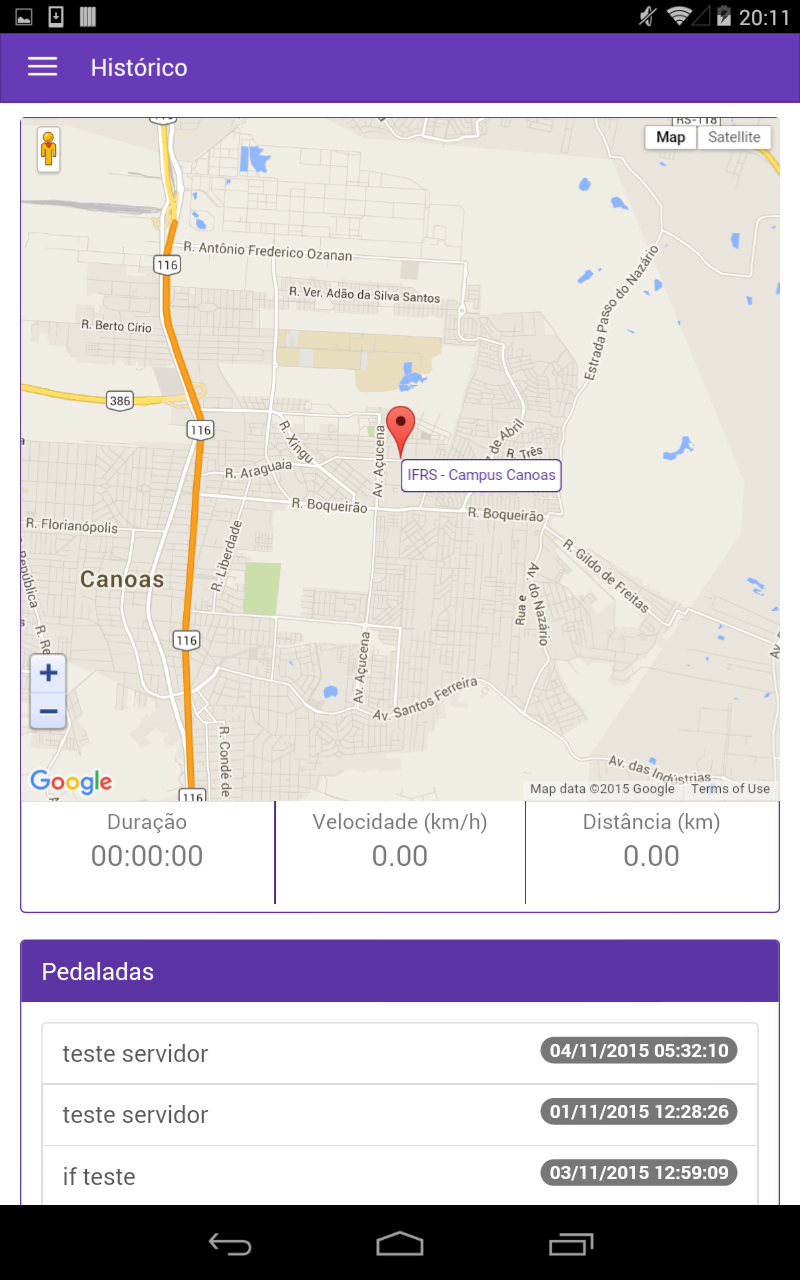
\includegraphics[width=0.95\linewidth]{figuras/p2pmaps.png}
    \label{fig:recordsMobile}
\end{minipage}%
\begin{minipage}{.7\textwidth}
    \centering
    \captionof{figure}{Histórico de pedaladas\\em telas grandes.}
    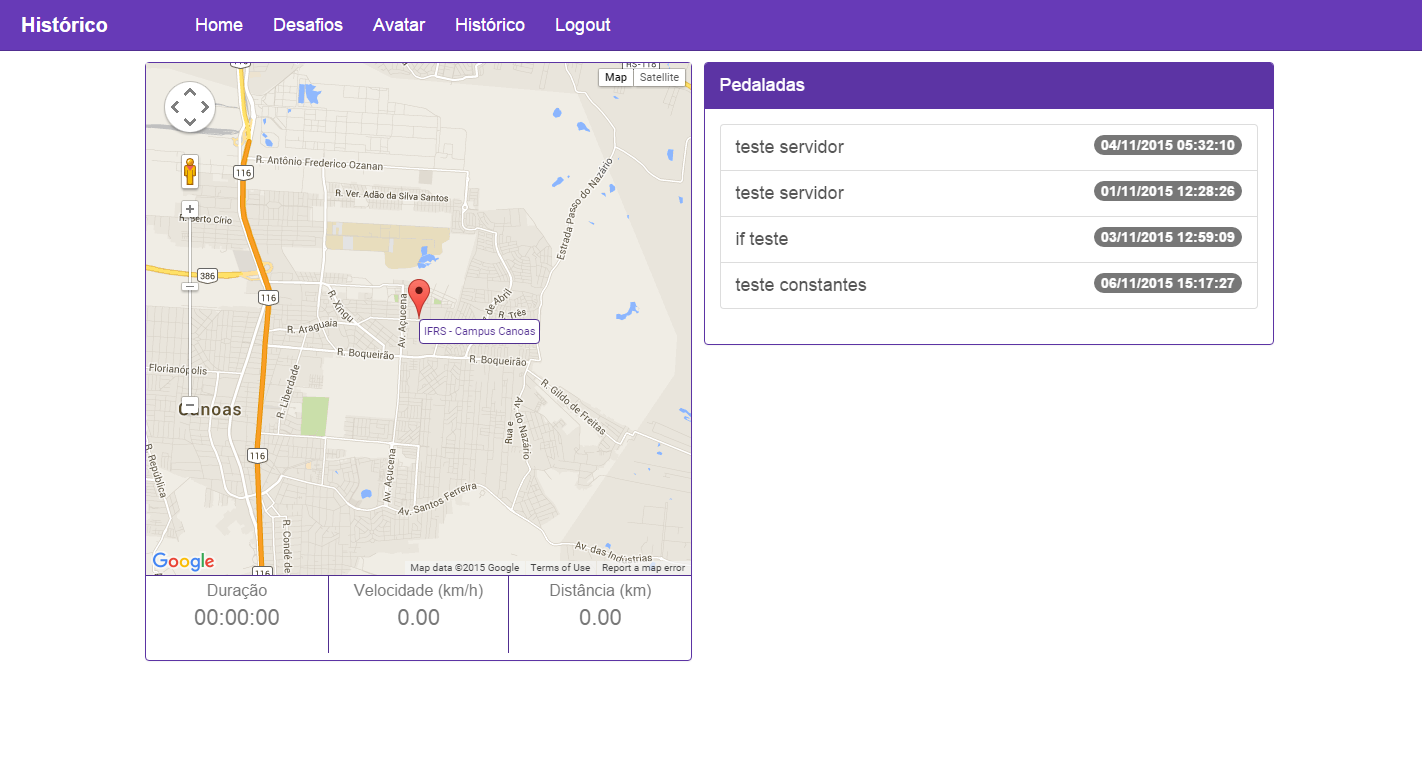
\includegraphics[width=1.1\linewidth]{figuras/p2pWebMaps.png}
    \label{fig:recordsWeb}
\end{minipage}
\par%
\bigskip
\centerline{Fonte: \textit{Print screens} do Pedal-to-Play.}
\end{figure}

Por último, a Figura \ref{fig:printMenu} apresenta o menu lateral desenvolvido usando o \textit{plugin} Jasny-Bootstrap. Este menu possibilita a navegação entre as GUI do Pedal-to-Play em telas com largura inferior a 768 \textit{pixels}. 

\begin{figure}[hb]
\begin{minipage}{.5\textwidth}
    \centering
    \captionof{figure}{GUI dos desafios.}
    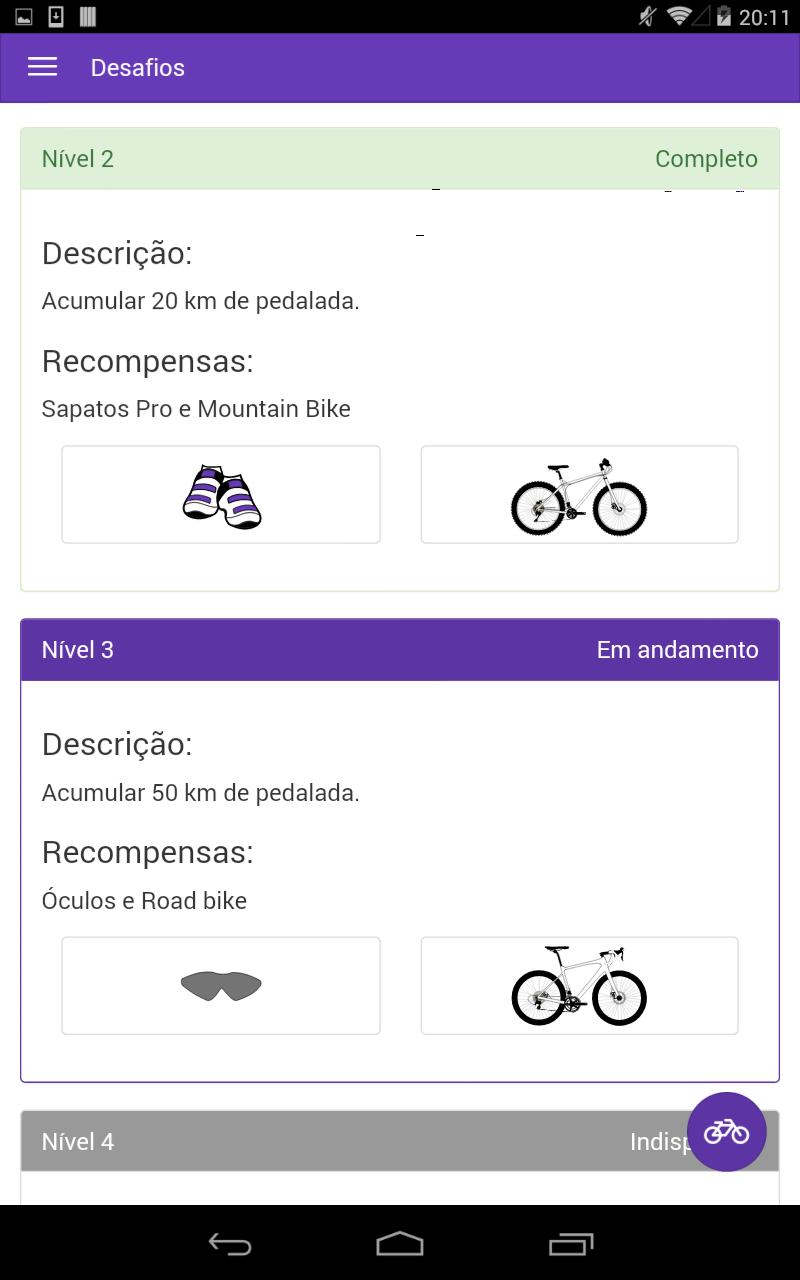
\includegraphics[width=0.5\linewidth]{figuras/p2pQuests.png}
    \label{fig:questsMobile}
\end{minipage}%
\begin{minipage}{.5\textwidth}
    \centering
    \captionof{figure}{Menu lateral para navegação.}
    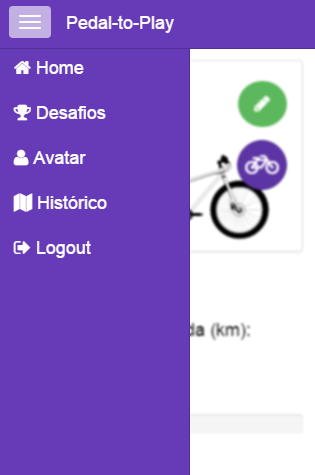
\includegraphics[width=0.5\linewidth]{figuras/p2pMenu.png}
    \label{fig:printMenu}
\end{minipage}
\par%
\bigskip
\centerline{Fonte: \textit{Print screens} do Pedal-to-Play.}
\end{figure}

\section{Teste do Monitoramento de Pedaladas}
Para verificação da funcionalidade de monitoramento de pedalada, utilizou-se os seguintes dispositivos com sistema operacional Android e com suporte à geolocalização, incluindo GPS:

\begin{enumerate}
\item Galaxy Fame Duos\footnote{\url{http://www.samsung.com/br/support/model/GT-S6812MBPZTM}}: é um modelo de \textit{smartphone} fabricado pela Samsung que conta com a versão Android 4.1.2 (Jelly Bean) e uma tela com resolução de 320 x 480 \textit{pixels}.

\item Moto G 2014\footnote{\url{http://www.motorola.com.br/Moto-G-da-Motorola/moto-g-2nd-gen-br.html}}: é um modelo de \textit{smartphone} fabricado pela Motorola que conta com a versão Android 4.4.4 (KitKat) e uma tela com resolução de 720 x 1280 \textit{pixels}.

\item Nexus 7 2012\footnote{\url{https://www.asus.com/Tablets/Nexus_7/}}: é um modelo de \textit{tablet} fabricado pela Asus que conta com a versão Android 4.4.4 (KitKat) e uma tela com resolução de 800 x 1280 \textit{pixels}.
\end{enumerate}

\subsection{Teste de Pedalada na Avenida Érico Veríssimo}
O primeiro teste ao ar livre realizado foi o monitoramento de uma pedalada rápida pela avenida Érico Veríssimo, no bairro Menino Deus, em Porto Alegre. O resultado deste teste é apresentado no mapa na Figura \ref{fig:trackErico}.

\begin{figure}[h]
\begin{minipage}{1.0\textwidth}
    \captionof{figure}{Monitoramento de pedalada na avenida Érico Veríssimo.}
    \centerline{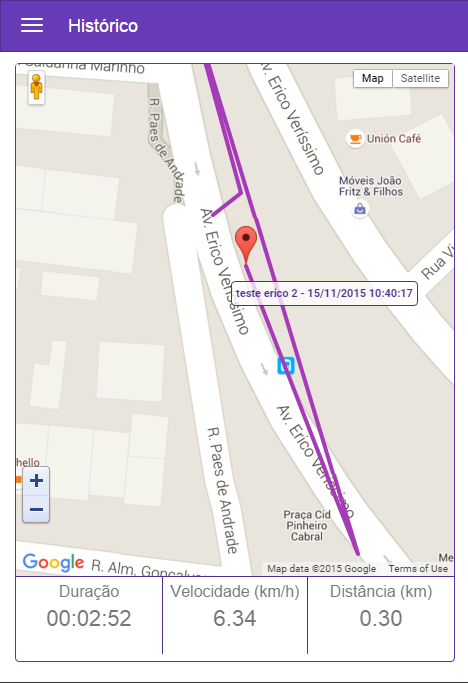
\includegraphics[width=13em]{figuras/p2pTrackErico.png}}
    \label{fig:trackErico}
\end{minipage}
\centerline{Fonte: \textit{Print screen} do Pedal-to-Play.}
\end{figure}

Como o monitoramento deste primeiro teste foi rápido, poucas posições foram capturadas pela API de geolocalização e por isso as linhas aparentam ser retas. As medidas totalizaram 300 metros de percurso, durante 2:52 minutos, resultando em uma velocidade média de 6,34 km/h. Este teste foi monitorado utilizando o Moto G.

\subsection{Teste de Pedalada no Parque Farroupilha}
O segundo teste ao ar livre foi o monitoramento de uma pedalada partindo do Parque Farroupilha até o estádio Olímpico, em Porto Alegre. O resultado deste teste é apresentado na Figura \ref{fig:trackRedencao}.

\begin{figure}[h]
\begin{minipage}{1.0\textwidth}
    \captionof{figure}{Monitoramento de pedalada no trajeto Parque Farroupilha-Olímpico.}
    \centerline{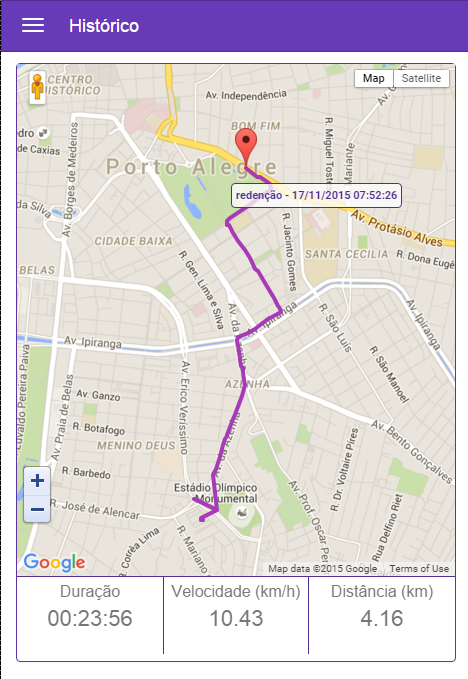
\includegraphics[width=11em]{figuras/p2pTrackRedencao.png}}
    \label{fig:trackRedencao}
\end{minipage}
\centerline{Fonte: \textit{Print screen} do Pedal-to-Play.}
\end{figure}

O teste totalizou 4,16 km de percurso, durante 23:56 minutos e uma velocidade média de 10,43 km/h. Por compreender uma pedalada mais longa do que o teste na Érico Veríssimo, o trajeto ficou mais detalhado no mapa. Para o monitoramento, utilizou-se o Galaxy Fame Duos.

\subsection{Teste sem Deslocamento}
O terceiro teste não foi ao livre e não envolveu deslocamento do usuário ou do dispositivo. O objetivo era analisar o comportamento da API de geolocalização enquanto o dispositivo está parado. Este teste foi realizado usando o Nexus 7 e seu resultado é apresentado na Figura \ref{fig:trackParado}.

\begin{figure}[h]
\begin{minipage}{1.0\textwidth}
    \captionof{figure}{\textit{Print screen} de um registro de monitoramento sem deslocamento.}
    \centerline{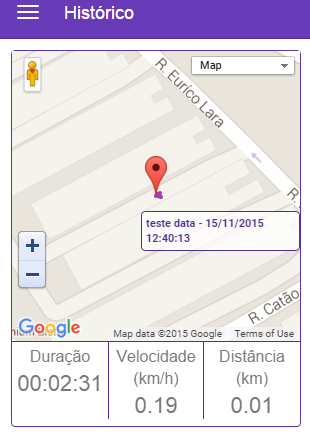
\includegraphics[width=10em]{figuras/p2pTrackParado.png}}
    \label{fig:trackParado}
\end{minipage}
\centerline{Fonte: \textit{Print screen} do Pedal-to-Play.}
\end{figure}

Como pode ser visto no \textit{print screen}, a aplicação quantificou um deslocamento de 10 metros, mesmo com o dispositivo parado. A justificativa para a API retornar posições diferentes quando não deveria é a existência de uma margem de erro, a qual é influenciada pela qualidade dos sensores no dispositivo e o nível do sinal deles. Os testes sem deslocamento foram realizados em ambientes fechados, o que compromete o sinal do GPS. Além disso, a especificação sobre Geolocalização da W3C\citeyearpar{w3cGeo} salienta que a posição retornada não tem garantia de ser verídica. Por estes fatores, trajetos curtos tendem a apresentar deformidades mais perceptíveis.
\par
O Strava detecta se o usuário está parado durante certo tempo e pausa a atividade para evitar deformidades no trajeto. Já o Runtastic não utiliza nenhum tratamento para esse fenômeno (ver teste na Figura \ref{fig:runtasticTesteParado}). 

\begin{figure}[hb]
\begin{minipage}{1.0\textwidth}
  \captionof{figure}{Registro de monitoramento sem deslocamento no Runtastic.}
  \centerline{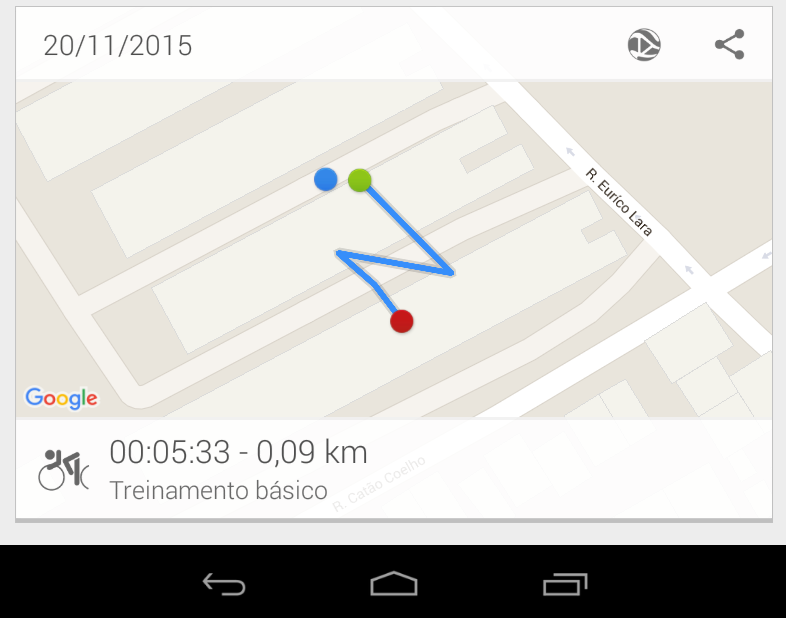
\includegraphics[width=.3\linewidth]{figuras/runtasticTesteParado.png}}
  \label{fig:runtasticTesteParado}
\end{minipage}
\par%
\bigskip
\centerline{Fonte: \textit{print screen} da aplicação Runtastic Road Bike.}
\end{figure}

% Conclusão
%Arquivo contendo o capítulo Conclusões
\chapter{Conclusão} \label{cap:conclusao}
Ao decorrer deste trabalho, dissertou-se sobre as etapas de desenvolvimento do projeto Pedal-to-Play. Inicia apresentando o cenário atual, no qual há uma ascensão do uso de dispositivos \textit{mobile} por toda a população e, em contrapartida, uma queda na prática de atividades físicas. Com a pretensão de unir estes dois mundos, o Pedal-to-Play tem o objetivo de proporcionar um ambiente motivador para a prática de atividades físicas com foco no ciclismo, por meio de um \textit{software} multiplataforma. O principal diferencial deste projeto em relação às outras aplicações existentes com o mesmo objetivo é a utilização de conceitos de gamificação (uso de elementos comuns em jogos para estimular a motivação do usuário). 
\par
Após definir os objetivos e apresentar a proposta do projeto, foram definidos os principais conceitos que permeiam o seu desenvolvimento. O conceito de jogo pervasivo, no qual uma parte da interação com o usuário transcorre no universo físico; de gamificação, explicado como a aplicação de mecanismos de jogos em contextos fora de jogos; de desenvolvimento multiplataforma, consistindo na utilização das tecnologias Web para a solução técnica do projeto; de avatares virtuais, o qual é um elemento comum em jogos digitais; de aplicativos de saúde e \textit{fitness}, referindo-se a categoria de sistemas com o objetivo de integrar tecnologia e atividades físicas e o conceito de geolocalização, consistindo nas técnicas implementadas para monitoramento da atividade do usuário.
\par
Também foram apresentados trabalhos na mesma temática, incluindo as aplicações comerciais Strava e Runtastic Road Bike, ambos possuindo a funcionalidade de monitoramento da atividade de ciclismo. Assim como trabalhos acadêmicos, como o de Cesani e Dranka, propondo um sistema de apoio aos ciclistas de Curitiba e o de Rosero, que desenvolveu soluções em \textit{hardware} e \textit{software} para apoio ao treinamento de ciclistas.
\par 
Contextualizado o sistema, a etapa seguinte envolveu a análise e o projeto da solução técnica. Consistiu na definição da arquitetura do sistema, seguindo o modelo Cliente-Servidor; no levantamento de requisitos, tanto funcionais, quanto não funcionais; na diagramação de casos de uso, definidos a partir dos requisitos funcionais; na prototipação das GUI e na diagramação do modelo de entidade e relacionamento. 
\par
A partir da análise e do projeto, iniciou-se a implementação da solução técnica. A implementação foi dividida em várias entregas e atividades, envolvendo o desenvolvimento dos módulos de Autenticação, de Monitoramento e registro de pedaladas, do Avatar virtual, de Desafios e as atividades de Compilação do projeto para plataforma Android e Hospedagem do \textit{web service} do Pedal-to-Play.
\par
Por fim, foram analisados os resultados obtidos a partir do desenvolvimento da solução técnica e testes monitorando pedaladas reais. Pôde-se afirmar que o Pedal-to-Play conseguiu cumprir grande parte de seus objetivos. A implementação de tecnologias Web permitiu suporte para vários dispositivos, o que conclui o objetivo de ser multiplataforma e de possuir uma interface responsiva, adaptável para diferentes tamanhos de tela. A API de geolocalização do \textit{framework} Cordova possibilitou o monitoramento das pedaladas do usuário e, consequentemente, a análise de dados como distância, tempo e velocidade, essenciais para determinar o desempenho do usuário e fornecer \textit{feedback}, completando o objetivo de analisar pedaladas. Os desafios, o avatar, o mecanismo de recompensas e níveis acrescentaram ao projeto a essência dos jogos e completaram o objetivo do sistema ser gamificado, promovendo a fuga da realidade e competição, os quais fazem parte dos principais fatores motivacionais do ser humano. A integração de todas estas funcionalidades e tecnologias implementadas no Pedal-to-Play tornaram-o um ambiente motivador e de entretenimento, tal qual ele pretendia ser.
\par
Como trabalhos futuros, as seguintes funcionalidades são interessantes para o sistema. A integração com redes sociais (a qual o projeto não conseguiu abordar) é interessante tanto para o usuário compartilhar suas realizações na aplicação (promovendo integração social e competição), quanto para o Pedal-to-Play promover-se nas redes sociais, atraindo mais usuários. A utilização da API do acelerômetro do Cordova, pois possibilitaria um controle mais refinado durante o monitoramento das pedalas, considerando que a geolocalização possui uma margem de erro, o acelerômetro pode ser usado como um complemento para determinar se o usuário está em movimento ou não ou até mesmo se ele está dentro de um veículo e não sobre uma bicicleta. A análise de viabilidade para integração com outras APIs de dados cartográficos, como o OpenStreetMap, pois a API do Google Maps consome uma quantidade significativa de dados de Internet e processamento, o que não é interessante para dispositivos \textit{mobile}. A disponibilidade de desafios compartilhados entre os usuários, como no Strava existem os segmentos, os quais consistem em trajetos no mapa disputados pelos usuários para determinar quem conseguirá os melhores resultados.
\par
E por fim, na parte "gamificada" do sistema, poderão ser desenvolvidos mais níveis, mais desafios (envolvendo diferentes medidas e objetivos), mais recompensas e mais peças para o avatar. Esta possibilidade é totalmente viável, levando em conta que o modo de implementação dos módulos permite dinamismo para acrescentar facilmente mais conteúdo ao sistema.

% carrega o arquivo com as bibliografias e põe o capítulo com as referências neste lugar
\bibliography{bibliografia}

% a partir daqui, todo capítulo novo é apêndice
\appendix

% Repositório e Versões
\chapter{Repositório e Versões}
O repositório no GitHub com o código-fonte e a documentação deste projeto se encontram na seguinte URL: \url{https://github.com/kaelvofraga/Pedal-to-Play}.
\par
A versão Web pode ser acessada pelo endereço \url{http://pedal2play.kaelfraga.com/} e a versão Android pode ser baixada em \url{https://bitbucket.org/kael_fraga/pedal2play/downloads/pedal2play.apk} ou via o QR Code da Figura \ref{fig:qrcode}.

\begin{figure}[hb]
\begin{minipage}{1.0\textwidth}
  \captionof{figure}{QR Code para \textit{download} da versão Android.}
  \centerline{
\includegraphics[width=.3\linewidth]{figuras/qrcode.png}}
  \label{fig:qrcode}
\end{minipage}
\end{figure}

%\chapter{Anexos e Apêndices}
%Destinam-se à inclusão de informações complementares ao trabalho, mas que não %são essenciais à sua compreensão. Os Apêndices devem apresentar material %desenvolvido pelo próprio autor, formatado de acordo com as normas. Já os %Anexos destinam-se à inclusão de material como cópias de artigos, manuais, %etc., que não necessariamente precisam estar em conformidade com o modelo, e %que não foram desenvolvidos pelo autor do trabalho.

%importa dicasLatexABNT.tex para o Apêndice 
%\chapter{Dicas de Latex e Normas ABNT}
Esta capítulo apresenta as coisas básicas que precisamos saber para fazer um TCC com Latex utilizando este modelo.

\section{O Básico do Latex}
Novo parágrafo pode ser feito por meio do comando par. \par
Outra forma é deixando uma linha em branco entre dois parágrafos.

Tudo o que está a direita de um \% é um comentário.
% Isto é um comentário
Para inserirmos o símbolo de porcento de forma proposital, precisamos colocar a barra invertida antes: 90\%.

Os caracteres \& \$ \# \% \_ \{ \} \^{} \~{} $\backslash$ são todos especiais e precisam ser escritos como comandos (com uma barra antes).
% tem um web app para ajudar a encontrar outros símbolos neste endereço: http://detexify.kirelabs.org/classify.html

Aspas são digitadas com duas crases no início e duas aspas simples no final: ``Texto entre aspas''

Estilos de fontes: \textbf{negrito}, \textit{itálico}, \textrm{romano}, \textsf{sans serif}, \texttt{maquina de escrever}, \textsc{caixa alta}.

Capítulos, seções e subseções são inseridas com:
\begin{verbatim}
\chapter{Um Capítulo} -> 1. Um Capítulo
\section{Uma Seção} -> 1.1 Uma Seção
\subsection{Uma Subseção} -> 1.1.1 Uma Subseção
\subsubsection{Uma Subsubseção} -> 1.1.1.1 Uma Subsubseção
\chapter*{Um Capítulo} -> Um Capítulo sem numeração
\end{verbatim}
Não se deve utilizar mais do que 4 níveis.

Ambientes são utilizados para definir uma região do texto que haverá tratamento especial:

\begin{verbatim}
O ambiente verbatin significa "ao pé da letra". 
Ex.: & $ # % _ { } ^ ~ $
\end{verbatim}

\begin{center}
O ambiente center escreve centralizado.
\end{center}

\begin{quote}
O ambiente quote é útil para fazer citações.
\end{quote}

Esta é a forma como se descreve itens:
\begin{description}
\item[Item 1] Isto significa uma coisa.
\item[Item 2] Este significa outra coisa.
\end{description}

Esta é a forma como se cita itens:
\begin{itemize}
\item Item 1;
\item Item 2.
\end{itemize}

E esta é a forma como se enumera itens:
\begin{enumerate}
	\item Qual a alternativa correta?
		\begin{enumerate}
			\item esta.
			\item ou esta.
		\end{enumerate}
\end{enumerate}

Fórmulas matemáticas são colocadas dentro de um ambiente matemático. Tudo neste ambiente é considerado elemento numérico e possui uma formatação diferente. Os comandos aceitos também podem mudar.

Equações matemáticas em destaque são inseridas da seguinte maneira:

% tem um web app para ajudar a fazer equações neste endereço: http://mathurl.com/
% ou aqui: http://webdemo.visionobjects.com/#/demo/equation
$$
x=\frac{-b\pm\sqrt{b^2-4ac}}{2a}.
$$

ou 

\begin{equation}
\begin{array}{rcl}
x_2 - x_1 &\geq& b_1 r_1\\
x_2 - x_1 &\geq& b_2 r_2\\
x_2 - x_1 &\geq& b_n r_m\\
b_1 + b_2 + ... + b_n &=& 1
\end{array}
\end{equation}

enquanto equações inline são feitas desta forma: $r_i (1\leq i \leq m)$.

\section{Convenções}
Escreva o título e os capítulos, seções, subseções, etc. sempre com a primeira letra de cada palavra importante em Maiúsculo e o restante em minúsculo. O Latex se encarregará de deixar tudo MAIÚSCULO onde for necessário.

Nenhuma seção deve ficar sem texto.

Utilize siglas para não ter de repetir muitas vezes o mesmo texto. Neste caso, na primeira ocorrência coloque o significado antes e a sigla entre parênteses (aproveitando também para adiciona-la à lista de siglas). Nas demais ocorrências, apenas coloque a sigla. 
Ex.: ...execução do algoritmo de  \textit{Threshold Accepting} (TA) sobre um circuito. A versão do algoritmo de TA utilizada...

Palavras em \textit{English} ou outra lingua estrangeira devem estar em itálico. Utilize \textbf{negrito} quando for necessário destacar alguma coisa.

\section{Figuras e Tabelas}

Todas as figuras e tabelas devem estar referenciadas no texto e com a descrição acima delas. Não são permitidos outros nomes tais como: quadro, imagem, etc.  Comece a descrição com letra maiúscula e faça o restante em minúscula (exceto siglas), terminando com um ponto final.

Se buscada em alguma obra publicada, a citação deve sempre aparecer. Pode ser colocada entre parênteses, como no exemplo da Figura \ref{fig:dsp2}, ou preferencialmente abaixo após a palavra "Fonte: ", como no exemplo da Tabela \ref{tab:comp1}. Observando que na LISTA DE FIGURAS/TABELAS a fonte/citação não deve aparecer.

É possível colocar as figuras de lado e também redimensiona-las através dos parâmetrosdo Latex, como nos exemplos das Figuras \ref{fig:dsp} e \ref{fig:dsp2}. Dê preferência por imagens vetoriais ou em PDF, para não perder qualidade. Procure deixar os textos das figuras com o mesmo tamanho das letras no restante do documento.

\begin{figure} % [h] -> utilize este parâmetro para forçar nesta posição
    \caption{Segundo a ABNT, a descrição deve ficar acima da figura}
    \centerline{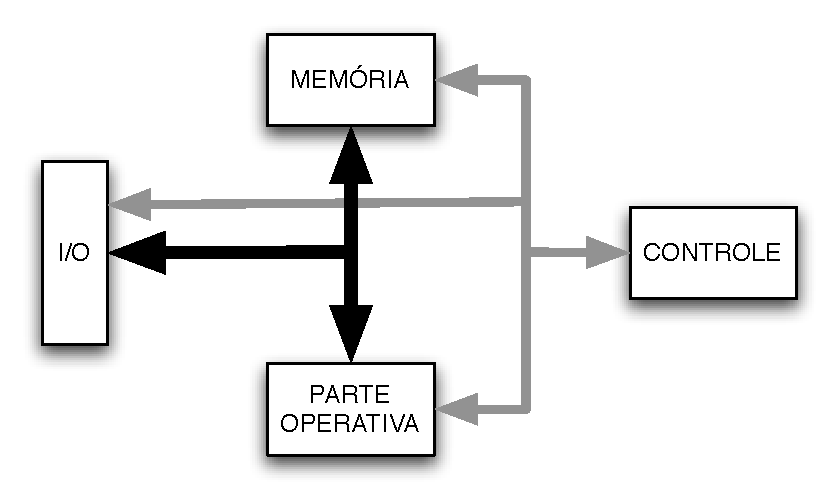
\includegraphics[width=20em]{figuras/dsp}}
    \label{fig:dsp}
\end{figure}

\begin{sidewaysfigure}
    % entre colchetes a descrição que vai para a lista de figuras, sem legenda (opcional)
    \caption[Descrição com citação]{Descrição com citação \cite{artigo}}
    \centerline{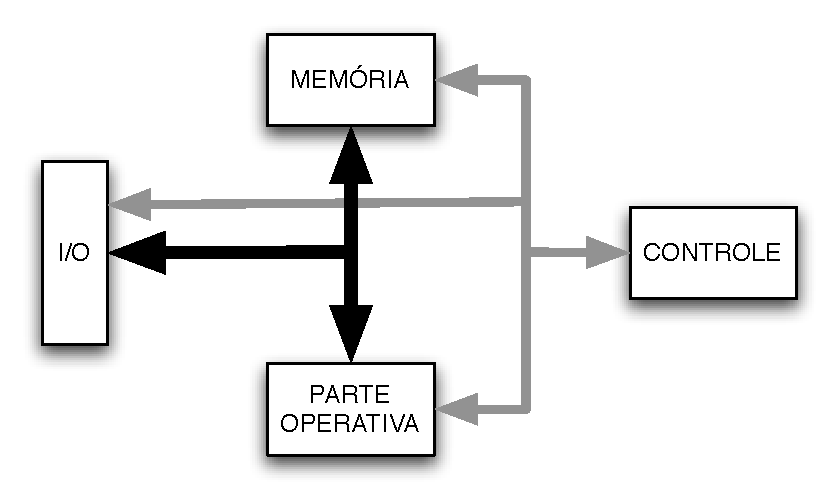
\includegraphics[width=40em]{figuras/dsp}}
    \label{fig:dsp2}
\end{sidewaysfigure}

As tabelas devem ser ``abertas'' dos lados (sem as linhas laterais), como no exemplo da Tabela \ref{tab:comp1}, isto torna a imagem mais limpa e clara.

% tem um web app para ajudar a fazer tabelas no latex neste endereço: http://truben.no/latex/table/
\begin{table}
    \centering
    \scalefont{0.93} %necessário eventualmente para reduzir o tamanho da tabela
    \caption{Comparação entre X e Y.}
    \begin{tabular}{c|c|c|c|c|c} \hline
        \multirow{2}{*}{\bf{Célula}} & \multirow{2}{*}{\# \bf{Trans.}} & \multicolumn{3}{|c|}{\bf{Largura} ($\mu m$)} & \bf{Tempo Exec. (s)}\\ \cline{3-6} 
         &  & Std. Cell & ASTRAN & \% & ASTRAN \\ \hline \hline
        AND2X4& 6 & 1 & 1,2 & 20 & 10 \\ \hline
        FAD1X4& 28 & 3,6 & 4 & 12 & 750\\ \hline
        FAD1X9& 28 & 4,2 & 4,2 & 0 & 1800\\ \hline
        HAD1X9& 14 & 2,4 & 2,4 & 0 & 30\\ \hline
        HAD1X18& 18 & 2,8 & 2,8 & 0 & 205\\ \hline
        INVX0 & 2 & 0,6 & 0,6 & 0 & 1\\ \hline
        TOTAL& - & 28 & 29 & 3,6 &-\\ \hline
    \end{tabular}
    {\\ Fonte: \cite{artigo}.}
    \label{tab:comp1}
\end{table}

\section{Citações}
Há duas formas de se fazer uma citação: a citação indireta ou livre e a citação direta ou textual. Todas as citações devem trazer a identificação de sua autoria.

No Latex, inserimos citações utilizando o formato bibtex. Para tanto, precisamos catastrar os dados da citação no arquivo .bib e em seguida citarmos no .tex com o comando cite. Colocar preferencialmente em ordem cronológica, com o mais recente por último \cite{livro, artigo, tese, capitulo, paper, site, apresentacao}.

\subsection{Citação Indireta}
Aquela citação na qual expressamos o pensamento de outra pessoa com nossas próprias palavras. Ex.:

Segundo o trabalho de Silva e Santos \citeyearpar{artigo}, o céu é azul porque...

O céu é azul porque... \cite{artigo}.

\subsection{Citação Direta}
São aquelas em que se transcreve exatamente as palavras do autor citado. As citações diretas ou textuais podem ser breves ou longas. São consideradas breves aquelas cuja extensão não ultrapassa três linhas e devem vir entre aspas. As citações com mais de três linhas são chamadas de longas (sem aspas) e devem receber um destaque especial com recuo.  Ex.:

Segundo Fulano, ``Quando a luz passa através de um prisma, seu espectro é dividido em sete cores monocromáticas'' \citeyearpar{artigo}.

\begin{quote}
Quando a luz passa através de um prisma, seu espectro é dividido em sete cores monocromáticas, eis que surge um arco-íris de cores. A atmosfera faz o mesmo papel do prisma, atuando onde os raios solares colidem com as moléculas de ar, água e poeira e são responsáveis pela dispersão do comprimento de onda azul da luz. \cite{artigo}
\end{quote}

Havendo supressão de trechos dentro do texto citado, faz-se a indicação com reticências entre colchetes [...]. De forma similar, para interpelação, acréscimo ou comentário durante a citação, deve-se fazê-lo também entre colchetes. No início ou no fim da citação, as reticências são usadas apenas quando o trecho citado não é uma sentença completa.Ex.:

``Também chamado de corpo do trabalho, [o desenvolvimento] tem por finalidade expor [...] a explicitação do assunto a ser abordado...'' \cite{artigo}.

\section{Notas de Rodapé}
As notas de rodapé\footnote{Nota sobre a palavra rodapé} são usadas nos documentos impressos para explicar ou fazer comentários detalhados.


\end{document}
